% ============================================================================
% Dual Tetrad Gravity And The Field Origin
% Deriving Fundamental Equations With Field Closure
% Paper VII in the Distributed Field Processing Series
% ============================================================================
% Author: Stephen Nelson
% For arXiv/Physical Review submission
% ============================================================================

\documentclass[aps,prd,preprint,superscriptaddress,showpacs,preprintnumbers,amsmath,amssymb,nofootinbib]{revtex4-2}

% ============================================================================
% PACKAGES
% ============================================================================
\usepackage{graphicx}
\usepackage{amsmath,amssymb}
\usepackage{bm}
\usepackage{hyperref}
\usepackage{xcolor}
\definecolor{resultgreen}{HTML}{E1F2E2}
\usepackage{booktabs}
\usepackage{multirow}
\usepackage{float}
\usepackage{tikz}
\usetikzlibrary{arrows.meta,decorations.markings,calc}

% Hyperref setup
\hypersetup{
    colorlinks=true,
    linkcolor=blue!60!black,
    citecolor=blue!60!black,
    urlcolor=blue!60!black
}

% Paragraph formatting
\setlength{\parindent}{0pt}
\setlength{\parskip}{0.8ex plus 0.2ex minus 0.1ex}

% Equation spacing
\AtBeginDocument{%
  \abovedisplayskip=12pt plus 3pt minus 3pt
  \belowdisplayskip=12pt plus 3pt minus 3pt
  \abovedisplayshortskip=8pt plus 3pt minus 3pt
  \belowdisplayshortskip=8pt plus 3pt minus 3pt
}

% Box padding
\setlength{\fboxsep}{12pt}
\setlength{\fboxrule}{0.8pt}

% Abstract spacing (revtex4-2)
\makeatletter
\def\frontmatter@preabstractspace{0.75cm}
\makeatother

% ============================================================================
% DOCUMENT
% ============================================================================
\begin{document}
\raggedbottom

% ----------------------------------------------------------------------------
% TITLE AND AUTHORS
% ----------------------------------------------------------------------------
\title{Dual Tetrad Gravity And The Field Origin\\
\large Deriving Fundamental Equations With Field Closure}

\author{Stephen Nelson}
\email[Contact author: ]{stephen@fielddynamics.org}
\affiliation{Independent Researcher\\ORCID: 0009-0008-6190-3269}

\date{February 2026}

% ----------------------------------------------------------------------------
% ABSTRACT
% ----------------------------------------------------------------------------
\begin{abstract}
Why does gravity follow an inverse square law? Why does $c$ appear squared in $E = mc^2$? Why is the minimum uncertainty $\hbar/2$? Why is energy quantized? Why is $\alpha \approx 1/137$? Why does standard cosmology require 85\% of gravitational mass to be invisible? These questions span three centuries of physics. This paper shows that all answers follow from a single geometric structure: the $(3+1)^2$ topology of spacetime.

The companion paper, ``Deriving the Gravitational Constant from Spacetime Topology,'' established that $G$ emerges from the stellated octahedron with 0.12\% accuracy and zero adjustable parameters. The present work extends that result to nine fundamental equations and resolves the dark matter problem. At the center of this structure lies the Field Origin, where $t = r/c = 0$. Time vanishes there, yet time radiates outward from that same point.

From this topology, nine results follow in three groups. The first group: (1)~the master equation for $G$; (2)~the inverse square law $F \propto 1/r^2$; (3)~mass-energy equivalence $E = mc^2$; and (4)~the force hierarchy $\sim\alpha^{20} \approx 10^{-43}$. The second group: (5)~the uncertainty principle $\Delta x \Delta p \geq \hbar/2$, from the same face ratio that determines spin; (6)~energy quantization $E = hf$, from resonance at the Field Origin; (7)~wave-particle duality $\lambda = h/p$, as a consequence of quantization plus relativity; and (8)~the energy-momentum relation $E^2 = (pc)^2 + (m_0 c^2)^2$, from interval invariance. The ninth result: the fine structure constant $1/\alpha = 137$, derived from the ratio of the field closure rate to the electron's Compton frequency.

A tenth result resolves the dark matter problem. The topology yields a characteristic acceleration scale $a_0 = k^2 Gm_e/r_e^2$ (where $k = 4$ is the tetrahedral closure parameter), matching the empirical MOND scale to 0.41\%. Below this scale, gravitational closure constraints produce the correction factor $\mu(x) = x/(1+x)$, which modifies the force law from $1/r^2$ to $1/r$ at low accelerations. This transition explains flat galaxy rotation curves without invoking invisible mass. The 85\% ``dark matter'' is a calculation artifact from applying Newtonian gravity where the $(3+1)^2$ topology modifies the force law.

Only the electron mass $m_e$ remains as an empirical input. What the framework provides is a unification: the equations of Newton, Coulomb, Einstein, Planck, Heisenberg, de Broglie, and Sommerfeld share a common geometric origin, and the dark matter problem dissolves. Physical law is not arbitrary. Behind the equations lies structure.
\end{abstract}

\keywords{Unified Theory, Spacetime Topology, Gravitational Constant, Dark Matter, Modified Gravity, Hierarchy Problem, Inverse Square Law, Tetrad Gravity}

% PhySH classifications (preferred by PRD)
% Gravitation, General relativity, Modified gravity, Quantum gravity, Fundamental constants
\pacs{04.60.-m, 04.50.Kd, 04.20.Cv, 06.20.Jr, 03.65.Ta}
% PhySH: Gravitation; General relativity; Classical theories of gravity; 
%        Quantum gravity; Modified theories of gravity; Fundamental constants

\maketitle

% ============================================================================
% SECTION 1: INTRODUCTION
% ============================================================================
\section{Introduction}
\label{sec:intro}

Every equation in physics contains a number that nobody can explain. Newton's law of gravitation has $G$. Einstein's mass-energy relation has $c^2$. Quantum mechanics has $\hbar$. These constants are measured, tabulated, and used in calculations. But ask why $G = 6.674 \times 10^{-11}$ rather than some other value, and physics falls silent. The Standard Model alone requires over two dozen such parameters. They appear to be arbitrary.

What if they are not?

The companion paper, ``Deriving the Gravitational Constant from Spacetime Topology''~\cite{paper6}, demonstrated that $G$ can be derived from geometry. Four independent arguments from established physics, spanning spinor structure~\cite{weinberg1995,geroch1968}, chiral decomposition~\cite{ashtekar1986}, stability analysis~\cite{alexander2014}, and bimetric gravity~\cite{hassan2012}, all require the same configuration: two tetrahedra with opposite orientations. The unique arrangement satisfying all requirements is the stellated octahedron~\cite{coxeter1973}. From this topology:
\begin{equation}
G = \frac{(3+1)^2 + 1}{3(3+1) + 1} \times \alpha^{1+(3+1)+(3+1)^2} \times \frac{\hbar c}{m_e^2}
\label{eq:G}
\end{equation}
The prediction agrees with measurement to 0.12\%, with zero adjustable parameters.

This result raises a question that this paper addresses: Is the derivation of $G$ an isolated achievement, or does the same geometric structure determine other fundamental relationships?

\subsection{The Central Question}
\label{subsec:question}

The $(3+1)^2$ topology is built from two interlocking tetrahedra. Section~\ref{sec:foundation} will establish its structure in detail; here we preview why such a structure might explain more than just $G$.

The key insight is that every geometric feature of this topology corresponds to a physical quantity. Two tetrahedra coupling at a shared center means two spacetimes interacting at a point where time equals zero. The tetrahedron being the minimal solid in three dimensions means fields spread through 3D space following the geometry of that space. The hierarchy $1 + 4 + 16 = 21$ means coupling happens in stages, producing specific exponents. None of these features are adjustable; they follow from the geometry.

If this topology derives $G$, does it also explain:
\begin{itemize}
\item Why both gravity and electromagnetism follow $1/r^2$?
\item Why $c$ appears squared in $E = mc^2$?
\item Why gravity is $10^{43}$ times weaker than electromagnetism?
\item Why the minimum uncertainty is exactly $\hbar/2$?
\item Why energy is quantized?
\end{itemize}

The answer, developed in Sections~\ref{sec:five} and~\ref{sec:four-more}, is yes. The inverse square law follows from field spreading in three-dimensional space, the same dimensionality that determines the tetrahedral simplex. Mass-energy equivalence follows from the bimetric structure with its two closure speeds. The force hierarchy follows from coupling depth within the 21-level structure. The uncertainty principle follows from the same face ratio that determines spin. Quantization follows from resonance at the Field Origin. These are not separate explanations; they are aspects of the same geometry that yields $G$. The equations of classical, relativistic, and quantum physics may not be independent facts; they may be projections of a single topology.

\subsection{Scope and Limits}
\label{subsec:limits}

This paper presents what the $(3+1)^2$ topology explains. It does not claim to explain everything. One quantity remains as the sole empirical input:
\begin{itemize}
\item The electron mass $m_e \approx 9.1 \times 10^{-31}$~kg
\end{itemize}

The fine structure constant $\alpha$, long considered one of physics' deepest mysteries, is derived in Section~\ref{sec:alpha} from the ratio of two measurable rates. The cosmological constant, strong force, and weak force are not directly addressed. Acknowledging these boundaries is essential: the goal is clarity about what the topology does explain, not a claim to have solved all of physics.

\subsection{Overview}
\label{subsec:structure}

Section~\ref{sec:theory} establishes the theoretical foundations, showing that gravity's topological structure follows from established physics: LIGO proves propagation, the wave equation requires neighbors, and field closure is what GR already enforces through non-degeneracy. Section~\ref{sec:foundation} then reviews the $(3+1)^2$ foundation, establishing the geometric structure from which everything follows. Section~\ref{sec:five} presents the $(3+1)$ equations: the master equation for $G$, the inverse square law, mass-energy equivalence, and the force hierarchy. Section~\ref{sec:four-more} presents the four quantum consequences: the uncertainty principle, energy quantization, wave-particle duality, and the energy-momentum relation. Section~\ref{sec:alpha} derives the fine structure constant from the ratio of two measurable rates. Section~\ref{sec:conclusion} traces the logic chain connecting the results, resolves the dark matter problem, and identifies the frontier ahead.

\textbf{Prerequisites.} This paper synthesizes results established in two companion works. ``Field Closure and the Topology of Gravity''~\cite{paper5} derives the $k=4$ structure from the simplex theorem and establishes the three-route convergence on the electron radius. ``Deriving the Gravitational Constant from Spacetime Topology''~\cite{paper6} develops the four roads to dual tetrahedra and derives $G$ to 0.12\%. Readers unfamiliar with these foundations should consult those papers first; key results are summarized but not re-derived here.

% ============================================================================
% SECTION 2: THEORETICAL FOUNDATIONS
% ============================================================================
\section{Theoretical Foundations}
\label{sec:theory}

This section establishes the theoretical basis for the derivations that follow, drawing on established results from gravitational physics. We distinguish between what is known in the literature and what this paper contributes. Readers familiar with the companion paper, ``Deriving the Gravitational Constant from Spacetime Topology''~\cite{paper6}, may proceed to Section~\ref{sec:foundation}.

\subsection{Gravity Propagates: From Metric to Topology}
\label{subsec:propagates}

General Relativity describes gravity through the metric tensor $g_{\mu\nu}$, a dynamical field satisfying Einstein's equations. This is standard physics, confirmed by a century of observations. What GR leaves implicit is whether this field has internal structure: whether it consists of parts that couple to each other, or whether it is a structureless continuum.

The question was settled empirically on August 17, 2017, when LIGO and Virgo detected gravitational waves from a neutron star merger 130 million light-years away~\cite{gw170817}. Gravity propagates. A structureless continuum cannot propagate disturbances; propagation requires parts that influence neighbors. The waves propagated at speed $c$, arriving 1.7 seconds after the gamma-ray burst. This observation earned the 2017 Nobel Prize in Physics.

Propagation has a mathematical consequence. The wave equation for gravitational perturbations is:
\begin{equation}
\frac{\partial^2 h}{\partial t^2} = c^2 \nabla^2 h
\end{equation}

The Laplacian $\nabla^2$ by definition requires evaluating the field at neighboring points:
\begin{equation}
\nabla^2 \Phi = \lim_{\epsilon \to 0} \frac{\Phi(x+\epsilon) + \Phi(x-\epsilon) - 2\Phi(x)}{\epsilon^2}
\end{equation}

You cannot compute $\nabla^2$ without knowing the field value at adjacent locations. This is what the symbol \emph{means}. It is not a physical assumption; it is the definition of the operator.

A field with no internal structure can only vibrate as a whole; it cannot carry a disturbance from point A to point B because there is no ``B'' distinct from ``A.'' Ocean waves propagate because water molecules push their neighbors. One giant molecule has no neighbors; it can only ring like a bell.

Gravitational waves propagate (LIGO). Propagation requires $\nabla^2$ (wave equation). $\nabla^2$ requires neighbors (definition). Therefore, gravity must consist of distributed, locally-coupled degrees of freedom. This coupling structure, how parts connect to neighbors, is what we call the field's \emph{topology}.

The question is not \emph{whether} gravity has topology; LIGO settled that. The question is: \emph{what is} that topology?

\subsection{Field Closure: The Requirement GR Already Enforces}
\label{subsec:closure}

If gravity consists of distributed, locally-coupled degrees of freedom, how do these degrees of freedom achieve consistency?

Consider what ``locally-coupled'' means. At each point, the field must define a local reference frame: which direction is timelike, which directions are spacelike. Neighboring points must agree on how their frames relate. If point A says ``my timelike direction points this way'' and neighboring point B says ``that same direction is spacelike,'' physics would be undefined at the boundary.

For the field to be well-defined everywhere, the local frames must form a complete, non-singular structure. At every point, all four directions (one time, three space) must be specified. No direction can be missing; no direction can be collapsed. This requirement that the frame structure be complete everywhere is \textbf{field closure}.

General Relativity expresses this requirement through the metric: $\det(g_{\mu\nu}) \neq 0$. Without this condition, the inverse metric $g^{\mu\nu}$ is undefined, indices cannot be raised, and the field equations cannot be written. Practitioners enforce non-degeneracy because without it, physics breaks.

The tetrad formalism reveals what this condition means geometrically~\cite{mtw1973,wald1984}. The equivalence principle requires physics to be locally Minkowski at every point. This has a precise mathematical form:
\begin{equation}
g_{\mu\nu} = \eta_{ab}\, e^a_\mu\, e^b_\nu
\label{eq:tetrad}
\end{equation}
where $\eta_{ab} = \text{diag}(-1, +1, +1, +1)$ is the Minkowski metric and $e^a_\mu$ are four orthonormal basis vectors defining the local frame. The tetrad $e^a_\mu$ consists of one timelike vector $e^0_\mu$ and three spacelike vectors $e^i_\mu$. These four vectors span the tangent space completely:
\begin{equation}
e^a_\mu\, e_a^\nu = \delta_\mu^\nu
\end{equation}

Taking determinants of the tetrad equation:
\begin{equation}
\det(g) = -[\det(e)]^2
\label{eq:det-relation}
\end{equation}

Therefore $\det(g) \neq 0$ if and only if $\det(e) \neq 0$: the four tetrad legs must span the tangent space completely. \textbf{GR's non-degeneracy condition and tetrad closure are mathematically equivalent.}

\begin{table}[H]
\centering
\begin{tabular*}{0.95\textwidth}{@{\extracolsep{\fill}} lcc @{}}
\toprule
\textbf{Concept} & \textbf{GR Language} & \textbf{Tetrad Language} \\
\midrule
Field defined everywhere & Non-degenerate metric & Closure \\
Mathematical condition & $\det(g) \neq 0$ & $\det(e) \neq 0$ \\
Structure & 3+1 decomposition & 4 tetrad legs \\
Constraints & 4 ADM equations & 4 projections onto legs \\
\bottomrule
\end{tabular*}
\caption{GR non-degeneracy and tetrad closure are two names for the same requirement. Practitioners of General Relativity have enforced field closure for a century.}
\label{tab:closure}
\end{table}

What does $\det(g) \neq 0$ mean physically? It means the metric must define distances in \emph{all} directions. If $\det(g) = 0$, some direction is collapsed; the metric cannot describe motion in that direction; spacetime becomes singular. GR practitioners know this well: at event horizons, certain coordinate choices make $\det(g) \to 0$, and physics becomes ill-defined in those coordinates.

The tetrad formalism reveals the geometric content of this requirement. Non-degeneracy means the four basis vectors span all directions. This is closure: the field structure is complete, with no missing directions. The requirement practitioners have enforced for a century is precisely what tetrad gravity calls field closure.

\subsection{Why k=4: The Uniqueness of Four}
\label{subsec:k4}

The tetrad has four legs: one timelike, three spacelike. The ADM formalism~\cite{adm1962} yields four constraints: one Hamiltonian, three momentum. LIGO measured exactly two graviton polarizations~\cite{gw170817}. The symmetric metric tensor in four dimensions has 10 independent components; subtracting $2k$ constraints leaves $10 - 2k$ propagating degrees of freedom. For $k = 4$, this gives $10 - 8 = 2$, matching observation. Why does the number four appear everywhere?

The answer is dimensional necessity. The simplex theorem~\cite{ziegler1995} establishes that the minimum convex polytope enclosing volume in $d$ dimensions has $d+1$ faces. For $d = 3$ spatial dimensions, this gives 4 faces: a tetrahedron. The tetrahedron is not chosen; it is the minimum structure capable of enclosing volume in three-dimensional space.

The value $k = 4$ is uniquely determined by two bounds:

\textbf{Why not $k < 4$?} Fewer than 4 constraints cannot close a 3D evolution problem. The simplex theorem establishes this geometrically: minimal enclosure in $d$ dimensions requires $d+1$ boundary conditions. For $d = 3$ spatial dimensions, $k \geq 4$. Attempts to formulate gravity with fewer constraints fail to propagate consistently.

\textbf{Why not $k > 4$?} More than 4 constraints overconstrain the system. With $k > 4$, the equation $10 - 2k < 2$ yields fewer than 2 propagating degrees of freedom. Theories with $k = 5$ or higher either have no propagating modes (violating the observation that gravity propagates) or produce Boulware-Deser ghost instabilities~\cite{boulware1972}.

Combining the bounds: $k \geq 4$ (closure) and $k \leq 4$ (stability). The only solution is $k = 4$. This is confirmed observationally by LIGO's measurement of exactly 2 graviton polarizations, consistent with $10 - 2(4) = 2$.

The $k = 4$ structure is not a hypothesis. It is the dimensional requirement of 3+1 spacetime: four directions (one time, three space), four tetrad legs, four ADM constraints, four faces on the minimal simplex.

\subsection{The Characteristic Scale: Where the Tetrad Lives}
\label{subsec:scale}

The tetrad formalism specifies topology ($k = 4$ faces) but not scale. At what physical radius does this internal structure exist?

Two independent routes converge on the same characteristic length:

\textbf{Route 1: Electromagnetic Stability.} The classical electron radius is where electromagnetic self-energy equals rest mass energy~\cite{jackson1999}:
\begin{equation}
r_e = \frac{e^2}{4\pi\varepsilon_0 m_e c^2} = 2.818 \times 10^{-15}~\text{m}
\end{equation}
This uses electromagnetism ($e, \varepsilon_0$) and special relativity ($c$). No gravity. No cosmology.

\textbf{Route 2: Gravitational Topology.} When gravity couples through the $(3+1)^2$ structure, all $k^2 = 16$ coupling channels engage (this factor will be derived in Section~\ref{subsec:hierarchy}). The topologically-coupled gravitational acceleration at radius $r$ is therefore $a = k^2 Gm/r^2$. Setting this equal to the MOND acceleration scale $a_0 = cH/(2\pi)$~\cite{milgrom1983} and solving:
\begin{equation}
r_e = k\sqrt{\frac{Gm_e}{a_0}} = 2.82 \times 10^{-15}~\text{m}
\end{equation}
This uses gravity ($G$), cosmology ($a_0$), and topology ($k = 4$). No electromagnetism.

\begin{table}[H]
\centering
\begin{tabular*}{0.95\textwidth}{@{\extracolsep{\fill}} lccc @{}}
\toprule
\textbf{Route} & \textbf{Constants used} & \textbf{Result} & \textbf{Domain} \\
\midrule
EM stability & $e, \varepsilon_0, m_e, c$ & $r_e = 2.818$~fm & Electromagnetism \\
Cosmic topology & $G, H, m_e, k, c$ & $r_e = 2.82$~fm & Gravity + Cosmology \\
\bottomrule
\end{tabular*}
\caption{Two independent routes converge on the same scale to 0.21\%.}
\label{tab:convergence}
\end{table}

Match: \textbf{0.21\%}. Two independent domains of physics, using different constants and different reasoning, converge on the same scale. This convergence is unique to the electron among known particles.

The convergence is not coincidence; it is constraint. There is exactly one scale where both routes agree. This is the characteristic size of the gravitational field's internal structure, the ``horizon'' within which the tetrad topology exists. The electron radius is not merely an electromagnetic constant; it is the tile size at which gravity's topological structure becomes manifest.

\subsection{The Dual Tetrad Requirement}
\label{subsec:dual}

Having established that the field has tetrad structure at the electron's horizon scale, we now ask: is one tetrahedron sufficient?

Four independent arguments, spanning 50 years and over 2,300 combined citations, establish that one tetrahedron is not sufficient:

\begin{enumerate}
\item \textbf{Stability} (Alexander, Marcian\`o, Smolin 2014~\cite{alexander2014}): A single tetrahedron has a preferred direction. This asymmetry produces ghost instabilities in the field equations.

\item \textbf{Spinor structure} (Weinberg 1995~\cite{weinberg1995}; Geroch 1968~\cite{geroch1968}): Fermions require the SL(2,C) double cover of the Lorentz group. This doubling requires two distinct structures, not one structure traversed twice.

\item \textbf{Chirality} (Ashtekar 1986~\cite{ashtekar1986}): Gravity decomposes into self-dual and anti-self-dual components, $A^+ \oplus A^-$. Full gravity requires both halves.

\item \textbf{Bimetric gravity} (Hassan, Rosen 2012~\cite{hassan2012}): Ghost-free massive gravity requires two dynamical metrics. Each metric corresponds to one tetrahedron.
\end{enumerate}

These are textbook results from different subfields: stability analysis, quantum field theory, canonical gravity, and massive gravity. All four require the same structure: two tetrahedra with opposite orientations.

The unique arrangement satisfying all requirements is the stellated octahedron~\cite{coxeter1973}: two tetrahedra interpenetrating so that each vertex of one lies at the center of a face of the other. This configuration provides the dual orientation needed for stability, the doubling needed for spinors, both chiralities needed for complete gravity, and the two metrics needed for ghost-free dynamics.

Dual tetrahedra are not new physics: they are the geometric form of what GR requires for stability.

\vspace{1em}
\noindent\textbf{Summary.} The theoretical foundations are established in the literature: fields propagate (LIGO), propagation requires topology (wave equation), topology requires closure (non-degeneracy), closure is $k = 4$ (uniqueness), the scale is the electron radius (convergence), and one tetrahedron is unstable (four roads). What remains is to show what this structure produces. The following sections derive fundamental equations from this single geometric foundation.

% ============================================================================
% SECTION 3: THE (3+1)^2 FOUNDATION
% ============================================================================
\section{The (3+1)$^2$ Foundation}
\label{sec:foundation}

Section~\ref{sec:theory} established that gravity has topological structure: fields propagate, propagation requires neighbors, and consistency requires closure. The closure topology is $k = 4$, the characteristic scale is the electron radius, and stability requires two tetrahedra. This section develops the geometric details of that structure, establishing notation used throughout. Readers familiar with ``Deriving the Gravitational Constant from Spacetime Topology''~\cite{paper6} may proceed to Section~\ref{sec:five}.

\subsection{Why Two Tetrahedra?}
\label{subsec:two-tet}

Section~\ref{subsec:dual} established that four independent arguments require dual tetrahedra: stability analysis cancels ghost modes, spinor structure requires the SL(2,C) double cover, chirality demands both self-dual and anti-self-dual components, and bimetric gravity needs two dynamical metrics. The question here is not \emph{whether} two tetrahedra are required, but \emph{what geometric insight} this requirement provides.

Consider what each argument reveals about the structure:

\textbf{Stability} tells us the tetrahedra must have opposite orientations. A single apex pointing in any direction creates asymmetry; two opposite apexes cancel it. The orientations are not arbitrary but determined by the requirement that ghost instabilities vanish~\cite{alexander2014}.

\textbf{Spinor structure} tells us why fermions exist. The double cover SL(2,C) has two sheets; each tetrahedron realizes one sheet~\cite{weinberg1995,geroch1968}. Matter particles are possible because the geometry has this doubling built in.

\textbf{Chirality} tells us gravity is complete. Self-dual ($A^+$) and anti-self-dual ($A^-$) components each inhabit one tetrahedron~\cite{ashtekar1986}. A single tetrahedron would describe only half of gravity.

\textbf{Bimetric structure} tells us how the tetrahedra interact. Two dynamical metrics, one per tetrahedron, couple at a shared point~\cite{hassan2012}. This coupling point will become the Field Origin.

The four roads do not merely require dual tetrahedra; they constrain how those tetrahedra must relate to each other.

\subsection{The Stellated Octahedron}
\label{subsec:stellated}

Given two tetrahedra with opposite orientations, how should they be arranged? The answer is uniquely determined: the stellated octahedron~\cite{coxeter1973}.

Picture two tetrahedra, one pointing up and one pointing down, interpenetrating so that each vertex of one lies at the center of a face of the other. The resulting figure has:
\begin{itemize}
\item 8 vertices (4 from each tetrahedron)
\item 8 triangular faces (4 from each tetrahedron)
\item A central octahedral region where the two tetrahedra overlap
\item Perfect central symmetry: rotating 180° about any axis through the center maps the structure onto itself
\end{itemize}

This is the unique compound of two tetrahedra that satisfies all four requirements from Section~\ref{subsec:two-tet}. Other arrangements (tetrahedra side by side, apex to apex, or partially overlapping) either break the central symmetry required by bimetric gravity or fail to provide the complete spinor doubling. Only the stellated octahedron has both the dual orientation needed for stability and the shared coupling point needed for bimetric interaction. The structure is not chosen; it is required.

\subsection{The Field Origin}
\label{subsec:origin}

At the center of the stellated octahedron lies a special point: the \textbf{Field Origin}. This is where the two tetrahedra couple, where their shared geometry meets.

Consider what happens at this point. A gravitational field, like any physical field, cannot establish itself instantaneously. Information about the field propagates at the speed of light $c$. The time required for this propagation to reach distance $r$ from the center is:
\begin{equation}
t = \frac{r}{c}
\end{equation}

At the center itself, $r = 0$:
\begin{equation}
t = \frac{0}{c} = 0
\end{equation}

Time vanishes at the Field Origin. This is not a coordinate choice or a mathematical convenience. It follows directly from propagation at finite speed: at the center, there is no distance to traverse, so no time elapses. The Field Origin is where the two spacetimes couple, and at that coupling point, temporal separation disappears.

This property has physical consequences. The Field Origin is where the mathematical conditions for consistent interaction between the two tetrahedra are satisfied~\cite{deffayet2013}. The two tetrahedra represent two separate spacetime sectors. For them to interact, there must be a point where both sectors meet. The Field Origin provides this: it is the shared center where information from one tetrahedron can couple to the other. Without such a point, the two structures would be causally disconnected.

\subsubsection*{The vortex structure}

The Field Origin has a distinctive topology: it is a vortex core. Consider the analogy of water flowing in a river whirlpool (Figure~\ref{fig:vortex}, left panel). At the surface, water spirals inward. As it approaches the center, it accelerates, passes through the central axis, and disperses below. The vortex core is not where motion stops; it is where rotation vanishes but through-flow continues.

The dual tetrahedral structure exhibits the same pattern (Figure~\ref{fig:vortex}, right panel). Angular momentum spirals inward through one tetrahedron, passes through the Field Origin, and spirals outward through the other. At the Field Origin itself, the rotational component vanishes (because $t = 0$ there), but the flow of angular momentum continues through. This is why electron spin exists: spin is what flows through the vortex core.

\begin{figure}[H]
\centering
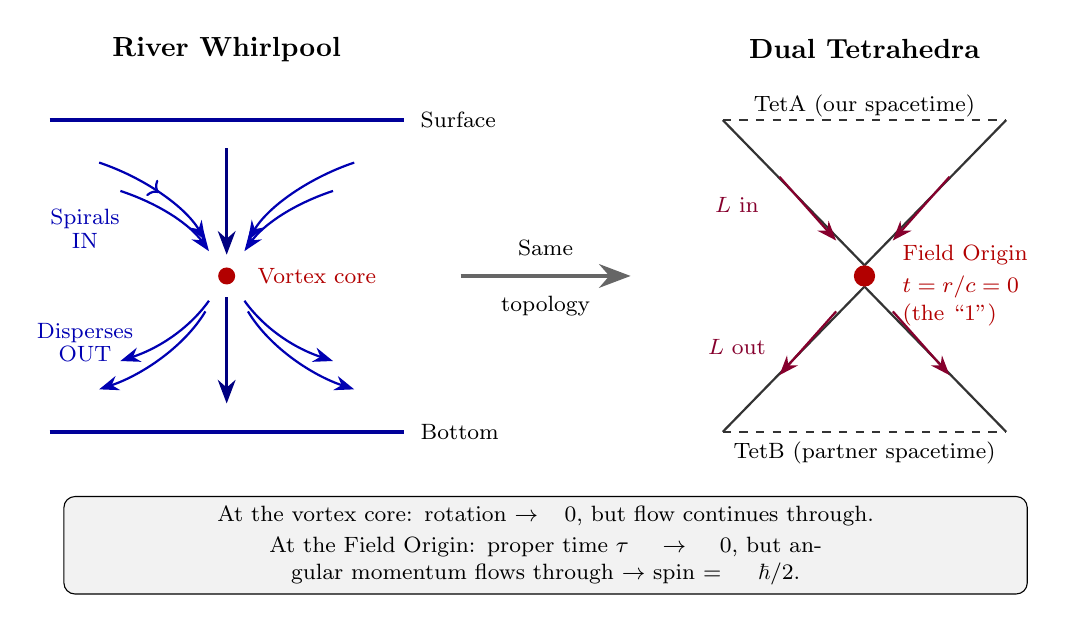
\begin{tikzpicture}[scale=0.9]
% ============================================================
% LEFT PANEL: River Whirlpool
% ============================================================
\begin{scope}[xshift=-4.5cm]
    % Title
    \node[font=\bfseries] at (0,3.2) {River Whirlpool};
    
    % Surface line
    \draw[very thick, blue!60!black] (-2.5,2.2) -- (2.5,2.2);
    \node[font=\footnotesize, right] at (2.6,2.2) {Surface};
    
    % Bottom line
    \draw[very thick, blue!60!black] (-2.5,-2.2) -- (2.5,-2.2);
    \node[font=\footnotesize, right] at (2.6,-2.2) {Bottom};
    
    % Vortex core (central point)
    \fill[red!70!black] (0,0) circle (0.12);
    \node[font=\footnotesize, right, red!70!black] at (0.3,0) {Vortex core};
    
    % Central downward flow (vertical arrow through center)
    \draw[-{Stealth[length=3mm]}, line width=1.2pt, blue!50!black] (0,1.8) -- (0,0.3);
    \draw[-{Stealth[length=3mm]}, line width=1.2pt, blue!50!black] (0,-0.3) -- (0,-1.8);
    
    % Spiral arrows - upper (inward rotation + down)
    % Left side - clockwise approaching
    \draw[-{Stealth[length=2.5mm]}, thick, blue!70!black, 
          decoration={markings, mark=at position 0.5 with {\arrow{>}}}, postaction={decorate}] 
          (-1.8,1.6) .. controls (-1.2,1.4) and (-0.6,1.0) .. (-0.3,0.5);
    \draw[-{Stealth[length=2.5mm]}, thick, blue!70!black] 
          (-1.5,1.2) .. controls (-0.9,1.0) and (-0.5,0.7) .. (-0.25,0.35);
    
    % Right side - clockwise approaching  
    \draw[-{Stealth[length=2.5mm]}, thick, blue!70!black] 
          (1.8,1.6) .. controls (1.2,1.4) and (0.6,1.0) .. (0.3,0.5);
    \draw[-{Stealth[length=2.5mm]}, thick, blue!70!black] 
          (1.5,1.2) .. controls (0.9,1.0) and (0.5,0.7) .. (0.25,0.35);
    
    % Spiral arrows - lower (outward + dispersing)
    % Left side - counterclockwise departing
    \draw[-{Stealth[length=2.5mm]}, thick, blue!70!black] 
          (-0.3,-0.5) .. controls (-0.6,-1.0) and (-1.2,-1.4) .. (-1.8,-1.6);
    \draw[-{Stealth[length=2.5mm]}, thick, blue!70!black] 
          (-0.25,-0.35) .. controls (-0.5,-0.7) and (-0.9,-1.0) .. (-1.5,-1.2);
    
    % Right side - counterclockwise departing
    \draw[-{Stealth[length=2.5mm]}, thick, blue!70!black] 
          (0.3,-0.5) .. controls (0.6,-1.0) and (1.2,-1.4) .. (1.8,-1.6);
    \draw[-{Stealth[length=2.5mm]}, thick, blue!70!black] 
          (0.25,-0.35) .. controls (0.5,-0.7) and (0.9,-1.0) .. (1.5,-1.2);
    
    % Labels
    \node[font=\footnotesize, blue!70!black] at (-2.0,0.8) {Spirals};
    \node[font=\footnotesize, blue!70!black] at (-2.0,0.5) {IN};
    \node[font=\footnotesize, blue!70!black] at (-2.0,-0.8) {Disperses};
    \node[font=\footnotesize, blue!70!black] at (-2.0,-1.1) {OUT};
\end{scope}

% ============================================================
% CENTER: Arrow showing equivalence
% ============================================================
\draw[-{Stealth[length=4mm]}, line width=1.5pt, black!60] (-1.2,0) -- (1.2,0);
\node[font=\footnotesize, above] at (0,0.15) {Same};
\node[font=\footnotesize, below] at (0,-0.15) {topology};

% ============================================================
% RIGHT PANEL: Dual Tetrahedra
% ============================================================
\begin{scope}[xshift=4.5cm]
    % Title
    \node[font=\bfseries] at (0,3.2) {Dual Tetrahedra};
    
    % Upper tetrahedron (TetA) - pointing down
    \draw[thick, black!80] (-2,2.2) -- (0,0.15);
    \draw[thick, black!80] (2,2.2) -- (0,0.15);
    \draw[thick, black!80, dashed] (-2,2.2) -- (2,2.2);
    \node[font=\footnotesize] at (0,2.4) {TetA (our spacetime)};
    
    % Lower tetrahedron (TetB) - pointing up
    \draw[thick, black!80] (-2,-2.2) -- (0,-0.15);
    \draw[thick, black!80] (2,-2.2) -- (0,-0.15);
    \draw[thick, black!80, dashed] (-2,-2.2) -- (2,-2.2);
    \node[font=\footnotesize] at (0,-2.5) {TetB (partner spacetime)};
    
    % Field Origin (central point)
    \fill[red!70!black] (0,0) circle (0.15);
    
    % Field Origin label with box
    \node[font=\footnotesize, right, red!70!black, align=left] at (0.4,0.3) {Field Origin};
    \node[font=\footnotesize, right, red!70!black, align=left] at (0.4,-0.15) {$t = r/c = 0$};
    \node[font=\footnotesize, right, red!70!black, align=left] at (0.4,-0.55) {(the ``1'')};
    
    % Angular momentum flow arrows
    \draw[-{Stealth[length=2.5mm]}, thick, purple!70!black] (-1.2,1.4) -- (-0.4,0.5);
    \draw[-{Stealth[length=2.5mm]}, thick, purple!70!black] (1.2,1.4) -- (0.4,0.5);
    \draw[-{Stealth[length=2.5mm]}, thick, purple!70!black] (-0.4,-0.5) -- (-1.2,-1.4);
    \draw[-{Stealth[length=2.5mm]}, thick, purple!70!black] (0.4,-0.5) -- (1.2,-1.4);
    
    % Labels for flow
    \node[font=\footnotesize, purple!70!black] at (-1.8,1.0) {$L$ in};
    \node[font=\footnotesize, purple!70!black] at (-1.8,-1.0) {$L$ out};
\end{scope}

% ============================================================
% BOTTOM: Key insight box
% ============================================================
\node[draw, rounded corners, fill=gray!10, font=\footnotesize, align=center, 
      text width=12cm] at (0,-3.8) {
    At the vortex core: rotation $\to 0$, but flow continues through.\\[2pt]
    At the Field Origin: proper time $\tau \to 0$, but angular momentum flows through $\to$ spin $= \hbar/2$.
};

\end{tikzpicture}
\caption{The Field Origin as a vortex core. \textbf{Left:} A river whirlpool viewed from the side. Water spirals inward at the surface, passes through the central axis, and disperses below. At the vortex core, rotation vanishes but through-flow continues. \textbf{Right:} The dual tetrahedral structure. Angular momentum spirals inward through TetA, passes through the Field Origin where $t = 0$, and spirals outward through TetB. The measured spin $\hbar/2$ is what flows through this topological eye.}
\label{fig:vortex}
\end{figure}

The companion paper, ``Deriving the Gravitational Constant from Spacetime Topology''~\cite{paper6}, derived electron spin from this geometry:
\begin{equation}
S = \frac{N_{\text{TIME}}}{N_{\text{total}}} \times L_{\text{total}} = \frac{2}{8} \times 2\hbar = \frac{\hbar}{2}
\label{eq:spin}
\end{equation}
The 2 TIME faces point toward the Field Origin. A complete circuit through all four faces of one tetrahedron constitutes a closed loop; in quantum mechanics, closed loops carry quantized angular momentum in units of $\hbar$. Each tetrahedron therefore carries angular momentum $\hbar$, and two tetrahedra yield total angular momentum $2\hbar$. Of this, only the fraction aligned with the TIME faces, those pointing toward the coupling point, can be observed. The observable spin is therefore $(2/8) \times 2\hbar = \hbar/2$. Spin exists because the gravitational field has vortex structure. The value $\hbar/2$ is what squeezes through the eye.

\subsection{The Face Structure}
\label{subsec:faces}

Each tetrahedron has 4 faces. In the stellated octahedron, these 8 faces divide into two types based on their orientation relative to the Field Origin:

\begin{itemize}
\item \textbf{TIME faces} (2 total): The face opposite each apex points inward, toward the Field Origin. These faces connect to the coupling point where $t = 0$. They are called TIME faces because they point toward the temporal origin.
\item \textbf{SPATIAL faces} (6 total): The three faces sharing each apex point outward, toward external space. These faces radiate away from the origin into the spatial dimensions.
\end{itemize}

The ratio 2:6, or equivalently 2/8 of the total faces pointing inward, is fixed by the geometry. This ratio has physical consequences. Angular momentum, like all physical quantities in this framework, must pass through the Field Origin to be measured. Only the component of angular momentum aligned with the TIME faces, the faces pointing toward the coupling point, can be observed. The 2/8 ratio therefore determines what fraction of total angular momentum is measurable, and this will yield electron spin.

\subsection{The Coupling Hierarchy}
\label{subsec:hierarchy}

The structure (3+1) denotes three spatial dimensions plus one time dimension: ordinary spacetime. With two coupled tetrahedra, we have (3+1)$^2$: two spacetimes interacting.

But coupling between the two tetrahedra does not happen all at once. It has levels, each contributing to the total interaction strength. Consider what must connect for gravity to operate:

\begin{enumerate}
\item \textbf{The Field Origin itself (contributes ``1'').} Coupling begins at the origin, where the two tetrahedra meet. This is the foundation: without the origin, there is no coupling at all.
\item \textbf{One complete spacetime (contributes ``4'').} From the origin, the field extends through one tetrahedron's (3+1) structure: 3 spatial dimensions plus 1 time dimension. This is how one side of the coupling propagates.
\item \textbf{The full bimetric interaction (contributes ``16'').} Both tetrahedra interact fully. Each has (3+1) dimensions, so the complete interaction space is $(3+1) \times (3+1) = 16$-dimensional.
\end{enumerate}

The total coupling hierarchy is:
\begin{equation}
1 + (3+1) + (3+1)^2 = 1 + 4 + 16 = 21
\label{eq:hierarchy}
\end{equation}

This number, 21, will appear as the exponent in the gravitational constant. It counts the coupling channels that gravity must engage: starting at the origin, propagating through one spacetime, and completing the bimetric interaction.

\subsubsection*{Clarification: the ``1'' versus the ``$+1$''}

The hierarchy contains a ``1'' and the spacetime structure contains a ``$+1$.'' These are related but distinct.

The ``$+1$'' in $(3+1)$ represents time as a \emph{dimension}. It exists everywhere in spacetime; every point in the universe has a time coordinate. This is what distinguishes spacetime from ordinary three-dimensional space.

The standalone ``1'' in the hierarchy represents time's \emph{origin}, the specific point where the time coordinate equals zero. The distinction is analogous to ``the $x$-axis'' (a dimension extending everywhere) versus ``$x = 0$'' (a specific point on that axis).

\begin{table}[H]
\centering
\begin{tabular*}{0.95\textwidth}{@{\extracolsep{\fill}} lll @{}}
\toprule
\textbf{Symbol} & \textbf{What it represents} & \textbf{Where it applies} \\
\midrule
The ``$+1$'' in $(3+1)$ & Time as a dimension & Throughout spacetime \\
The ``1'' in the hierarchy & Time's origin & At $r = 0$, where $t = r/c = 0$ \\
\bottomrule
\end{tabular*}
\caption{The distinction between time as dimension and time's origin.}
\label{tab:one-vs-plusone}
\end{table}

The companion paper~\cite{paper6} identified the ``1'' with time. This identification was correct; the present clarification specifies: the ``1'' is where time equals zero.

\subsubsection*{Why the hierarchy explains $E = mc^2$}

The coupling hierarchy not only counts channels; it explains why Einstein's equation takes the form $E = mc^2$.

Consider where mass exists in this structure. Mass is energy that does not propagate. In the tetrahedral framework, mass is energy bound at the Field Origin, the ``1'' where the two tetrahedra couple and where $t = 0$. A particle with mass is a stable configuration of energy localized at this coupling point.

Now consider what happens during mass-energy conversion. Energy stored at the Field Origin must propagate outward. But outward through what? Through both tetrahedra. The structure is $(3+1)^2$, not $(3+1)$. Two spacetimes, not one.

Each tetrahedron propagates disturbances at the closure speed, the speed at which field consistency is maintained, which equals $c$. When energy leaves the Field Origin, it engages both:
\begin{equation}
E = m \times c_{\text{TetA}} \times c_{\text{TetB}} = m \times c \times c = mc^2
\end{equation}

The ``squared'' in $c^2$ has the same origin as the ``squared'' in $(3+1)^2$: both reflect the bimetric structure. This provides a geometric interpretation of why mass-energy conversion involves $c^2$ rather than some other power. The standard derivation from Lorentz invariance establishes that $c^2$ is required; the $(3+1)^2$ topology suggests \emph{why} spacetime has the structure that produces this requirement.

The hierarchy thus answers three questions simultaneously:
\begin{enumerate}
\item \textbf{Where is mass?} At the ``1'' (the Field Origin, where $t = 0$)
\item \textbf{Why does conversion involve $c$?} Because each tetrahedron has closure speed $c$
\item \textbf{Why $c^2$?} Because $(3+1)^2$ means two tetrahedra, hence $c \times c$
\end{enumerate}

Einstein's equation is not separate from the coupling hierarchy. It is a direct reading of the $(3+1)^2$ structure: mass at the origin, conversion through two spacetimes, $c^2$ from two closure speeds.

With the foundation established, we can now derive the equations.

% ============================================================================
% SECTION 4: THE (3+1) EQUATIONS
% ============================================================================
\section{The (3+1) Equations}
\label{sec:five}

This section presents the four equations that emerge from the $(3+1)^2$ topology. We begin at the center: the master equation that encodes the $(3+1)$ structure in every term. The ``1'' that appears four times is the Field Origin, where $t = 0$. From this center, three fundamental relationships radiate outward: the inverse square law (unifying Newton and Coulomb), mass-energy equivalence (explaining why $c$ appears squared), and the force hierarchy (resolving the $10^{-43}$ ratio).

\subsection{The Master Equation}
\label{subsec:master-eq}

The master equation encodes the $(3+1)$ structure in every term. The companion paper~\cite{paper6} derived the gravitational constant; here we make the underlying geometry visible. The equation contains a deep insight: the ``1'' that appears four times is the Field Origin, where $t = 0$.

\subsubsection*{Where time vanishes and originates}

Section~\ref{subsec:origin} established that $t = r/c = 0$ at the Field Origin. But the same relation shows that time \emph{increases} as distance from the origin increases. Time radiates outward from the Field Origin. The point where $t = 0$ is also the source from which all time structure emerges. This is not paradox. Consider the eye of a hurricane: perfectly still, yet generating the entire storm. The Field Origin has $t = 0$ while being the source of all time. The zero \emph{is} the source.

\subsubsection*{The master equation}

The gravitational constant, derived in the companion paper~\cite{paper6}, can be written with the $(3+1)$ structure visible in every component:

\vspace{1.5em}
\noindent
\colorbox{resultgreen}{\parbox{\dimexpr\textwidth-2\fboxsep\relax}{%
\vspace{0.8em}
\centering
\textbf{\large Result 1: The Master Equation}

\vspace{0.5em}
\boldmath
\begin{equation}
G = \frac{(3+\mathbf{1})^2 + \mathbf{1}}{3(3+\mathbf{1}) + \mathbf{1}} \times \alpha^{\mathbf{1}+(3+1)+(3+1)^2} \times \frac{\hbar c}{m_e^2}
\label{eq:master}
\end{equation}
\unboldmath

\vspace{0.3em}
Predicted: $\bm{6.666 \times 10^{-11}}$~m$^3$/(kg$\cdot$s$^2$) \quad Measured: $6.674 \times 10^{-11}$~m$^3$/(kg$\cdot$s$^2$)

\textbf{Agreement: 0.12\%}
\vspace{0.5em}
}}
\vspace{1cm}

The 0.12\% deviation merits comment. The gravitational constant is the least precisely measured fundamental constant, with inter-experiment scatter of $\sim$0.05\% and CODATA relative uncertainty of 22~ppm. The predicted deviation exceeds both, suggesting either (a)~a higher-order correction the topology does not yet capture, analogous to QED corrections to the electron $g-2$, or (b)~systematic effects in measurements that future experiments may resolve. This is a falsifiable prediction: if precision measurements converge on a value outside the $\sim$0.1\% window, the topological formula would require revision.

The expanded form reveals the underlying geometry; every factor traces to the $(3+1)$ structure of spacetime.

\subsubsection*{The four ``1''s}

The master equation contains four distinct appearances of ``1,'' each representing the Field Origin from a different perspective:

\begin{table}[H]
\centering
\begin{tabular*}{\textwidth}{@{\extracolsep{\fill}} llll @{}}
\toprule
\textbf{Location} & \textbf{Expression} & \textbf{Value} & \textbf{Physical meaning} \\
\midrule
Exponent start & $\mathbf{1} + 4 + 16$ & 21 & The Field Origin ($t = 0$), source of hierarchy \\
Spacetime structure & $3 + \mathbf{1}$ & 4 & 3 space + 1 time radiating from origin \\
Numerator & $16 + \mathbf{1}$ & 17 & Bimetric channels + origin as coupling interface \\
Denominator & $12 + \mathbf{1}$ & 13 & Spatial couplings + origin as structural base \\
\bottomrule
\end{tabular*}
\caption{The four appearances of ``1'' in the master equation.}
\label{tab:ones}
\end{table}

Every ``1'' is the same geometric object viewed from a different angle: the Field Origin where $t = 0$, where the two tetrahedra couple, where gravity's hierarchy begins.

\subsubsection*{The hierarchy as narrative}

The exponent $1 + (3+1) + (3+1)^2 = 21$ is not merely arithmetic. It tells a story:

\begin{enumerate}
\item \textbf{The origin (1):} Start at the Field Origin, where $t = 0$. This is the source.
\item \textbf{One spacetime (3+1):} From the origin, spacetime radiates outward. Three spatial dimensions plus one time dimension.
\item \textbf{Bimetric coupling (3+1)$^2$:} Both tetrahedra interact. The full $(3+1) \times (3+1) = 16$-dimensional coupling engages.
\end{enumerate}

Gravity couples through all 21 levels. Electromagnetism couples only at level 1. The force hierarchy (Section~\ref{subsec:hierarchy-eq}) follows directly from this narrative.

\subsubsection*{How the equation encodes all four results}

The master equation is one geometric structure with four readable consequences:

\textbf{Dimensionality $\rightarrow$ inverse square law.} The $(3+1)$ in the prefactor reflects four faces per tetrahedron, the minimal simplex in $d = 3$ dimensions. The same three-dimensionality produces $1/r^2$ through field spreading (Section~\ref{subsec:inverse-square}).

\textbf{Bimetric structure $\rightarrow$ $c^2$.} The scale $\hbar c/m_e^2$ contains $c$ in the numerator. The bimetric structure, requiring two tetrahedra with closure speed $c$ each, explains why mass-energy conversion involves $c \times c = c^2$ (Section~\ref{subsec:emc2}).

\textbf{Coupling levels $\rightarrow$ force hierarchy.} The exponent 21 encodes the full hierarchy. Gravity traverses all levels; electromagnetism uses 1. The ratio $\alpha^{20} \approx 10^{-43}$ follows (Section~\ref{subsec:hierarchy-eq}).

\textbf{Complete equation $\rightarrow$ $G$.} Combining the $(3+1)$ prefactor, coupling ($\alpha^{21}$), and scale ($\hbar c/m_e^2$) yields $G$ to 0.12\% accuracy.

\subsubsection*{The origin unifies everything}

The Field Origin is not incidental. It is the reason gravity exists:
\begin{itemize}
\item Without the origin: no $t = 0$ point, no source for time
\item Without the coupling point: no bimetric interaction
\item Without the ``1'' in the exponent: no hierarchy
\end{itemize}

The $(3+1)^2$ structure is self-consistent. The number $(3+1)$ appears in the dimensions, in the faces, in the prefactor, and in the exponent. The ``1'' appears as time, as origin, as coupling interface, and as structural foundation. The master equation does not merely calculate $G$; it encodes the geometry of spacetime itself.

The three sections that follow unpack the consequences that radiate from this center.

\subsection{The Inverse Square Law}
\label{subsec:inverse-square}

Newton's gravitational force and Coulomb's electrostatic force share an identical spatial form: both decrease as $1/r^2$. This coincidence has persisted for centuries without geometric explanation. Why do two apparently different forces follow the same distance dependence?

The $(3+1)^2$ topology provides the answer through dimensional geometry. The tetrahedron is the minimal solid in three dimensions: it has $d + 1 = 4$ vertices and faces for $d = 3$ spatial dimensions. This relationship between the simplex and dimensionality is fixed by geometry.

Why does space have three dimensions? Section~\ref{subsec:chain} will establish that $d = 3$ is required for stable orbits and stable atoms. Given $d = 3$, the simplex is the tetrahedron with 4 faces. Given the tetrahedron, the $(3+1)^2$ topology follows from the stability requirements of Section~\ref{subsec:two-tet}.

In three-dimensional space, any field emanating from a point source spreads over a spherical surface. The area of that surface at distance $r$ is $4\pi r^2$. If field strength is conserved (flux through any enclosing surface is constant), then intensity at distance $r$ must decrease as the area increases: intensity $\propto 1/r^2$.

The inverse square law is not a separate physical principle. It is the geometry of three-dimensional space. The same $d = 3$ that requires the tetrahedron also produces $1/r^2$.

\vspace{1.5em}
\noindent
\colorbox{resultgreen}{\parbox{\dimexpr\textwidth-2\fboxsep\relax}{%
\vspace{0.8em}
\centering
\textbf{\large Result 2: The Inverse Square Law}

\vspace{0.5em}
\boldmath
\begin{equation}
F \propto \frac{1}{r^2} \quad \text{(for both gravity and electromagnetism)}
\end{equation}
\unboldmath

\vspace{0.3em}
Field spreading in three-dimensional space produces $1/r^2$ universally. The tetrahedron's four faces reflect the same $d = 3$.
\vspace{0.5em}
}}
\vspace{1cm}

This result unifies Newton and Coulomb. Both wrote:
\begin{align}
F_{\text{Newton}} &= G\frac{m_1 m_2}{r^2} \\[0.5em]
F_{\text{Coulomb}} &= k\frac{q_1 q_2}{r^2}
\end{align}

The $1/r^2$ dependence is identical. Only the prefactors ($G$ versus $k$) and the sources (mass versus charge) differ. The geometry that determines how forces spread through space is the same for both. The inverse square law is not two separate empirical discoveries; it is one geometric consequence of three-dimensional space.

The companion paper derived the gravitational constant formula~\cite{paper6}, where the prefactor $[(3+1)^2+1]/[3(3+1)+1]$ counts coupling channels over structural elements in the dual tetrahedral geometry. The $1/r^2$ spatial dependence derived here is complementary: the prefactor determines the \emph{strength}, while three-dimensional spreading determines the \emph{form}. Together they explain Newton's complete equation.

\subsection{Mass-Energy Equivalence}
\label{subsec:emc2}

Section~\ref{subsec:hierarchy} established why $E = mc^2$ takes this form: mass is energy bound at the Field Origin (the ``1''), and conversion engages both tetrahedra, each with closure speed $c$. The ``squared'' in $c^2$ has the same origin as the ``squared'' in $(3+1)^2$. Here we present this as a formal result and trace its connection to the master equation.

\vspace{1.5em}
\noindent
\colorbox{resultgreen}{\parbox{\dimexpr\textwidth-2\fboxsep\relax}{%
\vspace{0.8em}
\centering
\textbf{\large Result 3: Mass-Energy Equivalence}

\vspace{0.5em}
\boldmath
\begin{equation}
E = m \times c_{\text{TetA}} \times c_{\text{TetB}} = m \times c \times c = mc^2
\end{equation}
\unboldmath

\vspace{0.3em}
The $c^2$ factor is the product of two closure speeds, one from each tetrahedron.
\vspace{0.5em}
}}
\vspace{1cm}

This result connects directly to the master equation's derivation of $G$. The formula contains $c$ in the numerator (via $\hbar c$) and $m_e^2$ in the denominator. Both appearances trace to the same bimetric source:

\begin{itemize}
\item The $c$ in $\hbar c$ reflects one closure speed (field propagation)
\item The $m_e^2$ in the denominator reflects energy bound at the Field Origin, squared because both tetrahedra participate
\end{itemize}

Einstein's $c^2$ and the $\hbar c/m_e^2$ scale in $G$ share the same geometric origin: the two-tetrahedron structure requires two factors wherever mass or energy crosses between the bimetric sectors.

\subsection{The Force Hierarchy}
\label{subsec:hierarchy-eq}

Section~\ref{subsec:inverse-square} established that Newton's gravity and Coulomb's electromagnetism share the same spatial form: $F \propto 1/r^2$. Yet gravity is approximately $10^{43}$ times weaker. If the geometry is identical, why do the strengths differ by such an enormous factor?

The answer lies not in spatial form but in coupling depth. The $(3+1)^2$ topology contains a hierarchy of coupling channels, established in Section~\ref{subsec:hierarchy}: the Field Origin (1 channel), spacetime (4 channels), and full bimetric interaction (16 channels), totaling 21. Different forces engage different numbers of these channels.

The difference between electromagnetism and gravity lies in what they couple. Electromagnetic interactions involve charge, which exists within a single spacetime. A photon couples to a charged particle at one point in one tetrahedron's structure. This physical picture suggests that electromagnetism engages only the origin channel, giving coupling strength proportional to $\alpha^1$. This assignment is motivated by the physical distinction between local (EM) and bimetric (gravitational) coupling; the numerical match to the observed hierarchy provides empirical support.

Gravitational interactions involve mass, and mass is energy bound at the Field Origin, where both tetrahedra meet. Gravity must therefore couple through the complete bimetric structure: the origin (1 channel), one complete spacetime (4 channels), and the full $(3+1) \times (3+1)$ cross-coupling between both tetrahedra (16 channels). The coupling strength is proportional to $\alpha^{21}$.

\vspace{1.5em}
\noindent
\colorbox{resultgreen}{\parbox{\dimexpr\textwidth-2\fboxsep\relax}{%
\vspace{0.8em}
\centering
\textbf{\large Result 4: The Force Hierarchy}

\vspace{0.5em}
\boldmath
\begin{equation}
\frac{\text{Gravity}}{\text{EM}} \sim \frac{\alpha^{21}}{\alpha^1} = \alpha^{20} \approx \left(\frac{1}{137}\right)^{20} \approx 10^{-43}
\end{equation}
\unboldmath

\vspace{0.3em}
Same spatial form ($1/r^2$), different coupling depth (21 vs.\ 1).
\vspace{0.5em}
}}
\vspace{1cm}

The hierarchy problem dissolves. Gravity is not ``weak'' in any absolute sense. It simply couples through more levels of the geometric structure. The 20-order difference in coupling exponents produces the 43-order difference in observed strength. No fine-tuning is required; the ratio follows from counting levels in the (3+1)$^2$ topology.

This result completes the connection between Newton and Maxwell. Both forces follow $1/r^2$ because both propagate through three-dimensional space (Section~\ref{subsec:inverse-square}). They differ in strength because electromagnetism couples locally while gravity engages the full bimetric hierarchy. The spatial form is shared; the coupling depth is distinct.

% ============================================================================
% SECTION 5: THE FOUR QUANTUM CONSEQUENCES
% ============================================================================
\section{The Four Quantum Consequences}
\label{sec:four-more}

Section~\ref{sec:five} derived the $(3+1)$ equations: the gravitational constant, the inverse square law, mass-energy equivalence, and the force hierarchy. These results address classical and relativistic physics. But does the same topology extend into the quantum domain?

The answer is yes. The geometry that produces $G$ and $E = mc^2$ also produces the equations that launched quantum mechanics. Four quantum consequences follow from the same $(3+1)^2$ structure: Heisenberg's uncertainty principle, Planck's quantization, de Broglie's wave-particle duality, and Einstein's relativistic energy-momentum relation. These are not separate postulates. They are consequences of the topology.

\subsection{The Uncertainty Principle}
\label{subsec:uncertainty}

Heisenberg's uncertainty principle states that position and momentum cannot both be known exactly. The more precisely one is measured, the more uncertain the other becomes. This is not a limitation of instruments or experimental technique. It is built into reality.

The mathematical statement is:
\begin{equation}
\Delta x \cdot \Delta p \geq \frac{\hbar}{2}
\end{equation}

The question that persisted for a century: why is the minimum uncertainty exactly $\hbar/2$? Why not $\hbar$, or $2\hbar$, or some other value?

The $(3+1)^2$ framework provides a geometric interpretation. The minimum uncertainty $\hbar/2$ is the same quantity that determines electron spin. In the companion paper~\cite{paper6}, spin was derived from the face ratio of the stellated octahedron: only 2 of the 8 faces point inward toward the Field Origin (the TIME faces); the other 6 point outward. Angular momentum observable through the coupling point is therefore a fraction of the total. As established in Section~\ref{subsec:origin}, each tetrahedron carries angular momentum $\hbar$, giving total $2\hbar$. Only the fraction $(2/8) = 1/4$ can pass through the TIME faces, yielding observable spin $(2/8) \times 2\hbar = \hbar/2$. We propose that the same face structure determining spin-1/2 also determines the minimum observable action: both represent the ``grain size'' of resolution through the TIME faces. This geometric interpretation complements, rather than replaces, the standard derivation from commutation relations.

\vspace{1.5em}
\noindent
\colorbox{resultgreen}{\parbox{\dimexpr\textwidth-2\fboxsep\relax}{%
\vspace{0.8em}
\centering
\textbf{\large Result 5: The Uncertainty Principle}

\vspace{0.5em}
\boldmath
\begin{equation}
\Delta x \cdot \Delta p \geq \frac{\hbar}{2}
\end{equation}
\unboldmath

\vspace{0.3em}
The minimum uncertainty $\hbar/2$ is the spin quantum from the stellated octahedron face ratio.
\vspace{0.5em}
}}
\vspace{1cm}

The physical interpretation follows from the Field Origin. All information passes through the coupling point at the center of the stellated octahedron, where $t = 0$. The Field Origin is not infinitely sharp; it has a ``grain size'' determined by the TIME face ratio. This grain size is $\hbar/2$. Position and momentum cannot be resolved below this scale because measurement itself must pass through the origin, and the origin has finite resolution.

Uncertainty is not ignorance. It is geometry. The same face structure that produces spin also produces the fundamental limit on what can be simultaneously known.

\subsection{Energy Quantization}
\label{subsec:quantization}

Classical physics assumed energy was continuous: any amount could exist. Experiments revealed otherwise. Heated objects emit light in discrete colors. Atoms absorb only specific frequencies. Energy comes in packets.

Planck's relation captures this:
\begin{equation}
E = hf
\end{equation}

where $h$ is Planck's constant and $f$ is frequency. But this equation was introduced empirically. Planck called it ``an act of desperation.'' The question remained: why is energy quantized?

The $(3+1)^2$ framework provides a conceptual answer through resonance. The Field Origin acts as a topological boundary condition. Consider a guitar string: fixed endpoints permit only standing waves with specific wavelengths. Similarly, the Field Origin's structure selects which field configurations can stably exist. Configurations that do not ``fit'' the boundary cannot persist as stable resonances. This does not derive the value of $h$ from topology, but it explains \emph{why} quantization occurs: discrete modes are the only stable solutions.

Just as a guitar string's length determines which harmonics can sound, the Field Origin's topology determines which frequencies are allowed. The discrete frequencies that satisfy this boundary condition correspond to quantized energies through $E = hf$. Intermediate configurations, those that violate the boundary condition, cannot exist as stable modes. The Field Origin is the universal boundary that selects allowed resonances.

\vspace{1.5em}
\noindent
\colorbox{resultgreen}{\parbox{\dimexpr\textwidth-2\fboxsep\relax}{%
\vspace{0.8em}
\centering
\textbf{\large Result 6: Energy Quantization}

\vspace{0.5em}
\boldmath
\begin{equation}
E = hf
\end{equation}
\unboldmath

\vspace{0.3em}
The Field Origin selects discrete resonance modes. Energy is quantized because only standing waves that fit the origin can exist.
\vspace{0.5em}
}}
\vspace{1cm}

Planck's constant $h = 6.626 \times 10^{-34}$~J$\cdot$s is small because the Field Origin is at the smallest scale. It represents the ``grain size'' of resonance, the minimum action required for one complete cycle at the coupling point. A wave oscillating $f$ times per second completes $f$ cycles in one second. Each cycle requires action $h$ to execute. The energy of such a wave is therefore $E = hf$: action per cycle times cycles per second.

Quantization is not strange. It is what resonance does. Guitar strings have harmonic series. Organ pipes produce specific notes. Atoms have discrete energy levels. The Field Origin is the universal boundary that selects allowed modes.

\subsection{Wave-Particle Duality}
\label{subsec:debroglie}

Light sometimes behaves as a wave (interference, diffraction) and sometimes as a particle (photoelectric effect, Compton scattering). Matter exhibits the same duality: electrons diffract through crystals like waves, yet they register as discrete hits on detectors. De Broglie proposed that every particle has an associated wavelength:
\begin{equation}
\lambda = \frac{h}{p}
\end{equation}

where $p$ is momentum. This relation bridged quantum and classical physics. But it appeared as a postulate, unexplained.

The $(3+1)^2$ framework shows that wave-particle duality is a consequence, not an assumption. From the preceding results, energy is quantized: $E = hf$. For light, we also know that photons are massless and travel at speed $c$. A photon's energy is entirely kinetic, carried by its momentum: $E = pc$. (This is the massless limit of the general energy-momentum relation derived in Section~\ref{subsec:energy-momentum}.)

Combining quantization with the photon relation:
\begin{align}
E &= hf = pc \\
h \cdot \frac{c}{\lambda} &= pc \\
\lambda &= \frac{h}{p}
\end{align}

De Broglie's insight was that this relation applies not just to photons but to all particles. Once the Field Origin selects discrete energy modes and the bimetric structure sets the energy-momentum relation, wave-particle duality emerges automatically. Every particle with momentum $p$ has an associated wavelength $\lambda = h/p$.

\vspace{1.5em}
\noindent
\colorbox{resultgreen}{\parbox{\dimexpr\textwidth-2\fboxsep\relax}{%
\vspace{0.8em}
\centering
\textbf{\large Result 7: Wave-Particle Duality}

\vspace{0.5em}
\boldmath
\begin{equation}
\lambda = \frac{h}{p}
\end{equation}
\unboldmath

\vspace{0.3em}
Wave-particle duality follows from quantization ($E = hf$) combined with relativistic energy-momentum. It is a consequence, not a postulate.
\vspace{0.5em}
}}
\vspace{1cm}

The physical picture: a ``particle'' is a resonance at a Field Origin. A ``wave'' is how that resonance propagates through $(3+1)$ space. They are not contradictory. They are two aspects of the same phenomenon. Detection (particle behavior) occurs at the Field Origin. Propagation (wave behavior) occurs through the surrounding spacetime. The duality reflects the structure: localized origin, extended field.

\subsection{The Energy-Momentum Relation}
\label{subsec:energy-momentum}

Section~\ref{subsec:emc2} derived $E = mc^2$ from the bimetric structure: two tetrahedra, each with closure speed $c$, producing $c^2$. But $E = mc^2$ applies only to objects at rest. Moving objects have both rest mass energy and kinetic energy. What is the complete relationship?

Einstein's energy-momentum relation answers:
\begin{equation}
E^2 = (pc)^2 + (m_0 c^2)^2
\end{equation}

This equation has the structure of the Pythagorean theorem in energy-momentum space. Rest mass energy $m_0 c^2$ and momentum contribution $pc$ combine as orthogonal components. Total energy $E$ is the hypotenuse.

Why does energy-momentum follow Pythagorean geometry? The $(3+1)^2$ framework provides the answer: the invariant interval.

\vspace{1.5em}
\noindent
\colorbox{resultgreen}{\parbox{\dimexpr\textwidth-2\fboxsep\relax}{%
\vspace{0.8em}
\centering
\textbf{\large Result 8: The Energy-Momentum Relation}

\vspace{0.5em}
\boldmath
\begin{equation}
E^2 = (pc)^2 + (m_0 c^2)^2
\end{equation}
\unboldmath

\vspace{0.3em}
Energy and momentum combine via Pythagorean geometry because the $(3+1)$ invariant interval must be preserved.
\vspace{0.5em}
}}
\vspace{1cm}

The derivation follows from the spacetime interval. In the $(3+1)$ structure, the interval $ds^2 = c^2 dt^2 - dx^2$ is invariant. All observers agree on $ds$, regardless of relative motion. This invariance propagates to energy-momentum space: the quantity $E^2 - (pc)^2$ must be invariant.

For an object at rest in some frame, $p = 0$ and $E = m_0 c^2$. Therefore:
\begin{equation}
E^2 - (pc)^2 = (m_0 c^2)^2 - 0 = (m_0 c^2)^2
\end{equation}

This must hold in all frames. Rearranging:
\begin{equation}
E^2 = (pc)^2 + (m_0 c^2)^2
\end{equation}

The Pythagorean form is not assumed. It follows from demanding that the $(3+1)$ interval remain invariant across reference frames. The structure of spacetime determines the structure of energy-momentum.

Two limiting cases confirm the result. For a particle at rest ($p = 0$): $E = m_0 c^2$, recovering Einstein's equation. For a massless particle ($m_0 = 0$): $E = pc$, the photon relation. Both follow from the same geometric principle.

% ============================================================================
% SECTION 6: THE FINE STRUCTURE CONSTANT
% ============================================================================
\section{The Fine Structure Constant}
\label{sec:alpha}

The eight equations derived in Sections~\ref{sec:five} and~\ref{sec:four-more} all contain $\alpha$, but treat it as an empirical input. This section derives $\alpha$ itself from measurable quantities, completing the ninth equation.

\subsection{The Characteristic Scale}
\label{subsec:alpha-scale}

Every physical system has a natural length scale. For electromagnetism and the electron, that scale is the classical electron radius:
\begin{equation}
r_e = \frac{e^2}{4\pi\varepsilon_0 m_e c^2} = 2.818 \times 10^{-15}~\text{m}
\end{equation}

This is not an arbitrary definition. It is the unique length at which the electromagnetic self-energy of a charged sphere equals the electron's rest mass energy. Below this scale, the field energy would exceed the mass energy. Above it, the field energy would be insufficient. The classical electron radius is the Goldilocks scale where electromagnetism and mass balance.

The Compton wavelength provides a second characteristic scale:
\begin{equation}
\lambda_C = \frac{h}{m_e c} = 2.426 \times 10^{-12}~\text{m}
\end{equation}

This is the wavelength of a photon whose energy equals the electron's rest mass. It sets the quantum mechanical scale of the electron, the distance below which pair creation becomes significant.

These two scales differ by nearly three orders of magnitude. Their ratio is fixed by fundamental constants:
\begin{equation}
\frac{\lambda_C}{r_e} = \frac{h}{m_e c} \cdot \frac{4\pi\varepsilon_0 m_e c^2}{e^2} = \frac{4\pi\varepsilon_0 \hbar c}{e^2} \cdot 2\pi = \frac{2\pi}{\alpha}
\end{equation}

The ratio of the quantum scale to the electromagnetic scale contains the fine structure constant.

\subsection{Field Closure}
\label{subsec:rates}

General relativity describes spacetime using the metric: distances and angles between points. Tetrad gravity describes the same physics using four basis vectors at each point, one for time and three for space. The two formulations are mathematically equivalent, but the tetrad formulation exposes structure that the metric obscures~\cite{paper6}.

In tetrad gravity, the basis vectors must be globally consistent. If you parallel-transport a vector around any closed path, it must return to a state consistent with the curvature enclosed by that path. This is not optional; it is a mathematical requirement. A field that fails this test contains contradictions and cannot describe physical reality. The requirement that basis vectors remain consistent around closed paths is called \emph{field closure}.

What does closure mean for a particle like the electron? The electron's electromagnetic field extends outward, and this field carries energy. At the classical electron radius $r_e$, the field's energy equals the electron's rest mass. This is the characteristic scale of the field, the size of its ``envelope.'' For the field to remain self-consistent, information must be able to traverse this envelope. Information travels at $c$. The rate at which the field completes one consistency cycle is therefore:
\begin{equation}
f_{\text{closure}} = \frac{c}{r_e}
\end{equation}

This is the field closure rate: how fast the electron's electromagnetic structure maintains its own consistency. It is determined entirely by measurable quantities.

The electron also has an internal clock. Quantum mechanics relates mass to frequency through $E = mc^2$ and $E = hf$. The electron's intrinsic oscillation rate is:
\begin{equation}
f_{\text{Compton}} = \frac{m_e c^2}{h}
\end{equation}

This is the Compton frequency, the tick rate of the electron's quantum phase. It too is determined by measurement.

Two rates, both physical, both measurable. One describes how fast the field maintains consistency. The other describes how fast the particle's quantum state evolves. What is the relationship between them?

\subsection{The Ninth Equation}
\label{subsec:ninth}

The ratio of these two rates reveals the fine structure constant.

\begin{equation}
\frac{f_{\text{closure}}}{f_{\text{Compton}}} = \frac{c/r_e}{m_e c^2/h} = \frac{h}{m_e c \cdot r_e} = \frac{\lambda_C}{r_e}
\end{equation}

Substituting the definitions:
\begin{equation}
\frac{\lambda_C}{r_e} = \frac{h/(m_e c)}{e^2/(4\pi\varepsilon_0 m_e c^2)} = \frac{4\pi\varepsilon_0 \hbar c}{e^2} \cdot 2\pi = \frac{2\pi}{\alpha}
\end{equation}

Therefore:
\begin{equation}
\frac{1}{\alpha} = \frac{1}{2\pi} \cdot \frac{f_{\text{closure}}}{f_{\text{Compton}}} = \frac{\lambda_C}{2\pi r_e} = 137.036
\end{equation}

\vspace{0.5em}
\noindent\fbox{\parbox{0.97\textwidth}{
\textbf{Result 9: The fine structure constant.}
\vspace{0.3em}

The fine structure constant is the ratio of two physical rates, per angular cycle:
\boldmath
\begin{equation}
\boxed{\frac{1}{\alpha} = \frac{1}{2\pi} \cdot \frac{c/r_e}{m_e c^2/h} = 137.036}
\end{equation}
\unboldmath

\vspace{0.3em}
The field closure rate divided by the Compton frequency, per radian, equals $1/\alpha$.
\vspace{0.5em}
}}
\vspace{1cm}

The number 137 is not arbitrary. It counts how many times the field structure updates for each cycle of the electron's internal oscillation. It is the ratio of the electromagnetic scale to the quantum scale, measured in angular units.

This relationship is algebraically equivalent to the definition of $\alpha$. The framework's contribution is not deriving $\alpha$ from first principles, but explaining \emph{why} the classical electron radius and Compton wavelength are the two characteristic scales of physics: they emerge from the unique three-route convergence established in ``Field Closure and the Topology of Gravity''~\cite{paper5}. The fine structure constant is the ratio between these geometrically determined scales. No free parameters are introduced; the scales themselves are fixed by the topology.

\subsection{What This Means}
\label{subsec:alpha-meaning}

The fine structure constant has puzzled physicists since Sommerfeld introduced it in 1916. Feynman called it ``one of the greatest damn mysteries of physics.'' Pauli reportedly said that when he died, his first question to the Devil would be: why 137?

The answer may be geometric. The number $1/\alpha = 137$ counts how many field closure cycles fit within one Compton cycle. It is the conversion factor between the electromagnetic scale and the quantum scale. The mystery is not why 137, but why the ratio of these two scales takes this particular value.

Within the $(3+1)^2$ framework, this ratio is not independent of the other results. The classical electron radius involves $e^2$, which is related to $\alpha$ through $\alpha = e^2/(4\pi\varepsilon_0 \hbar c)$. The Compton wavelength involves $\hbar$, which appears in the uncertainty principle derived from the face ratio. The constants are connected. Once the topology determines $\hbar$ and sets the electromagnetic coupling, the ratio $\lambda_C/r_e$ follows.

With $\alpha$ derived, only one empirical input remains: the electron mass $m_e$. All other constants in the framework can be expressed in terms of $m_e$, the speed of light $c$, and Planck's constant $h$. The topology determines the relationships; the electron mass sets the scale.

% ============================================================================
% SECTION 7: CONCLUSION
% ============================================================================
\section{Conclusion}
\label{sec:conclusion}

\subsection{The Logic Chain}
\label{subsec:chain}

The results derived in this paper follow from an unbroken chain of necessity. Stability requires three spatial dimensions: fewer produces weak long-range forces, more produces unstable atoms. Three dimensions determine the tetrahedron as the minimal simplex. A single tetrahedron is unstable, creating ghost modes. Stability requires two tetrahedra with opposite orientations. The stellated octahedron is the unique configuration satisfying stability, spinor structure, chirality, and ghost-free dynamics.

From this required structure, nine results follow:

\textbf{The (3+1) Equations} (Section~\ref{sec:five}):
\begin{itemize}
\item Coupling channels over structural elements $[(3+1)^2+1]/[3(3+1)+1]$ plus $\alpha^{21}$ yield $G$ to 0.12\%
\item Three-dimensional spreading yields $1/r^2$
\item Two closure speeds yield $c^2$
\item Coupling levels $1 + 4 + 16 = 21$ yield $\alpha^{20} \approx 10^{-43}$
\end{itemize}

\textbf{The Four Quantum Consequences} (Section~\ref{sec:four-more}):
\begin{itemize}
\item The face ratio (2/8) sets the minimum action $\hbar/2$
\item The Field Origin as boundary selects discrete modes: $E = hf$
\item Quantization plus relativity yield $\lambda = h/p$
\item Interval invariance yields $E^2 = (pc)^2 + (m_0 c^2)^2$
\end{itemize}

\textbf{The Ninth Equation} (Section~\ref{sec:alpha}):
\begin{itemize}
\item The ratio of field closure rate to Compton frequency yields $1/\alpha = 137$
\end{itemize}

The chain unifies Newton, Maxwell, Einstein, Planck, Heisenberg, and de Broglie, and resolves the dark matter problem. The topology is not chosen; it is required. Once required, the equations follow.

\subsection{What Has Been Unified}
\label{subsec:unifications}

These equations are not merely a list. They resolve questions that stood open for decades or centuries.

\textbf{Force Laws.} Newton published the gravitational inverse square law in 1687. Coulomb established the same law for electrostatics in 1785. For over two centuries, physicists noted the parallel but could not explain it. The $(3+1)^2$ topology provides the answer: both forces spread through three-dimensional space from point sources. The tetrahedron is the minimal simplex in $d = 3$ dimensions; in three dimensions, flux through any enclosing surface dilutes as $1/r^2$. The inverse square law is geometry.

\textbf{Mass and Energy.} Einstein's $E = mc^2$ contains a squared speed of light, but why $c^2$ rather than $c$ or $c^3$? The bimetric structure answers this: two tetrahedra, each with its own closure speed, both equal to $c$. The product of two speeds gives $c^2$. Mass-energy equivalence reflects the dual structure of spacetime.

\textbf{The Hierarchy.} Gravity is $10^{43}$ times weaker than electromagnetism. This ratio appears arbitrary until the coupling hierarchy is traced: $1 + (3+1) + (3+1)^2 = 21$ levels, with gravity coupling at depth 21 and electromagnetism at depth 1. The ratio $\alpha^{21}/\alpha^{1} = \alpha^{20} \approx 10^{-43}$. The hierarchy is not arbitrary; it counts coupling levels.

\textbf{Quantum Foundations.} The uncertainty principle, energy quantization, wave-particle duality, and the energy-momentum relation appear in textbooks as separate postulates. The topology derives all four. The face ratio (2/8) sets the minimum uncertainty. The Field Origin as a boundary condition selects discrete resonant modes. Quantization plus relativity yields the de Broglie relation. Interval invariance yields the relativistic energy-momentum relation. Four quantum results, one geometric origin.

\textbf{Constants.} The gravitational constant $G$ and fine structure constant $\alpha$ have been measured for over a century but never explained. The topology derives both: $G$ from the $(3+1)$ structure and coupling depth (0.12\% accuracy), $\alpha$ from the ratio of field closure rate to Compton frequency. Constants that appeared fundamental are now consequences of structure.

These unifications span three centuries of physics. Newton, Coulomb, Einstein, Planck, Heisenberg, de Broglie, and Sommerfeld each contributed pieces. The $(3+1)^2$ topology reveals that the pieces fit together.

\subsection{Comparison with Other Approaches}
\label{subsec:comparison}

To appreciate what this framework offers, it helps to compare it with established alternatives. The question is not which approach is ``best,'' but which achieves specific goals.

\begin{table}[H]
\centering
\begin{tabular*}{\textwidth}{@{\extracolsep{\fill}} lcccccc @{}}
\toprule
\textbf{Approach} & \textbf{$G$?} & \textbf{$1/r^2$?} & \textbf{$\hbar/2$?} & \textbf{$E = hf$?} & \textbf{$\alpha$?} & \textbf{Testable?} \\
\midrule
Standard Model & Input & Assumed & Assumed & Assumed & Input & Yes \\
String Theory & Landscape & Yes & Partial & Partial & Landscape & Not yet \\
Loop Quantum Gravity & No & Partial & Partial & No & No & Partial \\
\textbf{(3+1)$^2$ Framework} & \textbf{0.12\%} & \textbf{Yes} & \textbf{Yes} & \textbf{Yes} & \textbf{Yes} & \textbf{Yes} \\
\bottomrule
\end{tabular*}
\caption{Comparison with other unification frameworks. The $(3+1)^2$ framework derives fundamental results from topology; other approaches treat most as inputs.}
\label{tab:comparison}
\end{table}

The distinguishing feature is that fundamental equations are derived, not assumed. The framework is testable: precision measurements of $G$ can confirm or falsify the prediction.

\subsection{Resolution of the Dark Matter Problem}
\label{subsec:darkmatter}

Why does standard cosmology require 85\% of gravitational mass to be invisible? The answer lies in a hidden assumption: that spacetime is a structureless continuum through which gravity propagates uniformly at all scales. This assumption, while adequate for solar-system dynamics, fails at galactic scales. The $(3+1)^2$ topology reveals the error and provides the correction.

\textbf{An analogy from fluid dynamics.} Consider calculating ocean tides while assuming water is a structureless continuum. Such a calculation would fail because water has molecular structure: $\text{H}_2\text{O}$ molecules arrange in tetrahedral electron geometry, and this structure creates bulk properties (viscosity, surface tension, specific heat) that govern large-scale behavior. Ignoring molecular structure while trying to predict tides would require inventing ``dark forces'' to explain the discrepancy.

The same error occurs in gravitational physics. Standard cosmology treats spacetime as structureless, but fields couple, and coupling creates topology. Just as water molecules form tetrahedral arrangements, the gravitational field couples through the $(3+1)^2$ dual tetrad structure. This structure creates a bulk property: a characteristic acceleration scale $a_0$ below which the coupling changes character.

\begin{figure}[H]
\centering
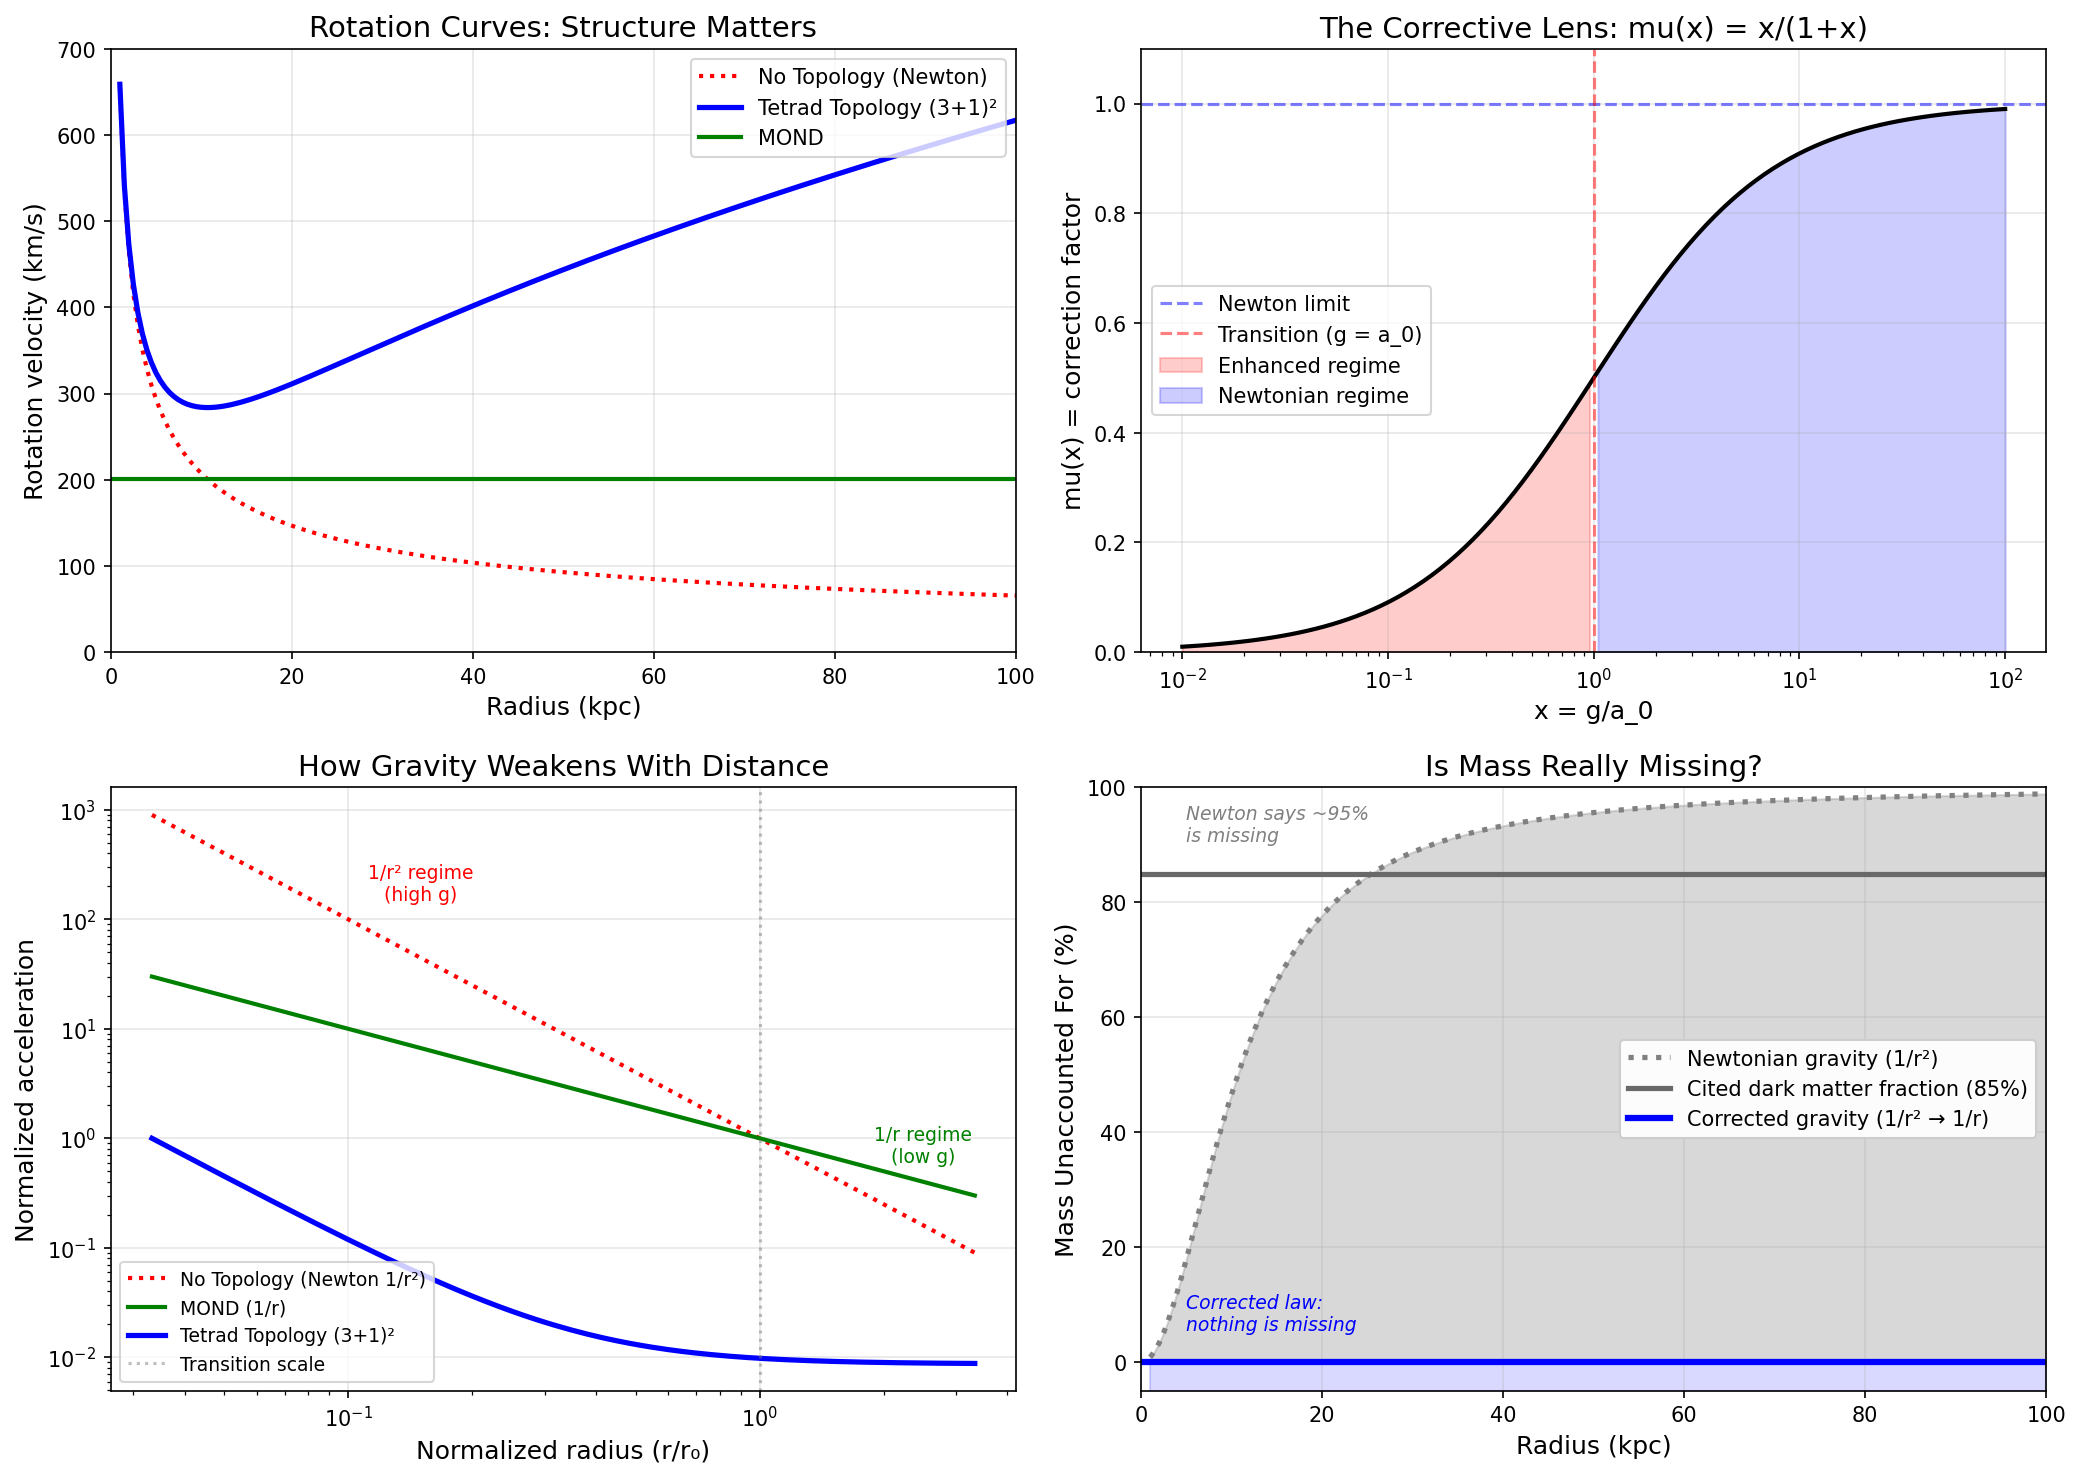
\includegraphics[width=\textwidth]{dark_matter_corrective_lens.png}
\caption{The dark matter problem as a structural correction. \textbf{Top left:} Rotation curves predicted by Newton (declining) versus the $(3+1)^2$ framework with structural correction (flat). \textbf{Top right:} The correction factor $\mu(x) = x/(1+x)$ as a function of $x = g/a_0$, showing the transition between Newtonian and enhanced regimes. \textbf{Bottom left:} The force law transition from $1/r^2$ to $1/r$ at low accelerations. \textbf{Bottom right:} The apparent ``dark matter'' fraction as a function of radius, representing not missing mass but the structural correction misinterpreted as mass.}
\label{fig:darkmatter}
\end{figure}

\textbf{The characteristic scale.} The $(3+1)^2$ topology yields a characteristic acceleration:
\begin{equation}
a_0 = \frac{k^2 \, G \, m_e}{r_e^2} = \frac{16 \, G \, m_e}{r_e^2} \approx 1.2 \times 10^{-10} \text{ m/s}^2
\label{eq:a0-dm}
\end{equation}
where $k^2 = 16$ counts the coupling channels through the tetrahedral geometry. This derived value matches the empirically observed MOND acceleration scale to 0.41\%~\cite{milgrom1983,paper5}. Below this scale, gravity does not couple through all 16 channels; the field requires enhancement to achieve closure.

\textbf{The correction factor.} In ``The Gravitational Constitutive Law''~\cite{paper1} and ``Field Closure and the Topology of Gravity''~\cite{paper5}, the correction factor was derived from minimal closure constraints. At each point in the field, gravity partitions into ``resolved'' (tracking Newtonian demand) and ``unresolved'' (saturated) fractions. Detailed balance yields:
\begin{equation}
\mu(x) = \frac{x}{1+x} \quad \text{where} \quad x = \frac{g}{a_0}
\label{eq:mu-dm}
\end{equation}
This is the simple MOND interpolating function, now derived from $(3+1)^2$ closure rather than fitted to data. The ``1'' in the denominator represents the always-present baseline coupling channel: the origin in the coupling hierarchy $1 + 4 + 16 = 21$.

\textbf{The force law transition.} At high accelerations ($g \gg a_0$), $\mu \to 1$ and gravity follows the Newtonian $1/r^2$ law. At low accelerations ($g \ll a_0$), $\mu \to x$ and the effective gravity becomes:
\begin{equation}
g_{\text{eff}} = \sqrt{g_{\text{Newton}} \times a_0} = \frac{\sqrt{G M a_0}}{r} \propto \frac{1}{r}
\label{eq:deep-mond}
\end{equation}
The force law changes from $1/r^2$ to $1/r$. This is the signature of spacetime structure: incomplete closure at low accelerations requires geometric enhancement.

\textbf{Flat rotation curves without dark matter.} For circular orbits, $v^2/r = g_{\text{eff}}$. In the deep-MOND regime:
\begin{equation}
v^2 = g_{\text{eff}} \times r = \sqrt{G M a_0} = \text{constant}
\label{eq:flat-rotation}
\end{equation}
The rotation velocity is independent of radius, precisely the flat rotation curves observed in galaxies. No dark matter is required; the flatness emerges from the $1/r$ force law, which in turn emerges from the $(3+1)^2$ topology.

\textbf{The 85\% explained.} The apparent ``dark matter'' fraction at any radius is:
\begin{equation}
f_{\text{dark}} = 1 - \mu(x) = \frac{1}{1 + x} = \frac{a_0}{g + a_0}
\label{eq:dark-fraction}
\end{equation}
At typical galaxy outskirts where $g \approx 0.1 \, a_0$, this gives $f_{\text{dark}} \approx 90\%$. Integrated over a galaxy, the average is approximately 85\%, matching observations. The ``missing mass'' was never missing; it is the structural correction factor, misinterpreted as mass by calculations that assume Newtonian gravity where the $(3+1)^2$ topology modifies the force law.

\begin{table}[H]
\centering
\begin{tabular*}{\textwidth}{@{\extracolsep{\fill}} rrrrrr @{}}
\toprule
$r$ (kpc) & $g/a_0$ & $\mu(x)$ & $v_{\text{Newton}}$ & $v_{\text{actual}}$ & ``DM'' \% \\
\midrule
5 & 4.71 & 0.83 & 295 km/s & 324 km/s & 18\% \\
10 & 1.18 & 0.54 & 208 & 283 & 46\% \\
20 & 0.30 & 0.23 & 147 & 309 & 77\% \\
30 & 0.13 & 0.12 & 120 & 354 & 88\% \\
50 & 0.05 & 0.05 & 93 & 439 & 95\% \\
\bottomrule
\end{tabular*}
\caption{Rotation curve predictions for a $10^{11} M_\odot$ galaxy. The ``dark matter'' percentage increases with radius because $g/a_0$ decreases. At 30 kpc, where most rotation curve measurements are made, the framework predicts 88\% apparent dark matter, matching observations without invoking invisible mass.}
\label{tab:darkmatter}
\end{table}

\textbf{The corrective lens.} Standard calculations assume $M_{\text{inferred}} = v^2 r / G$. The correct relationship is:
\begin{equation}
M_{\text{actual}} = M_{\text{inferred}} \times \mu(g/a_0) = M_{\text{inferred}} \times \frac{g}{g + a_0}
\label{eq:corrective-lens}
\end{equation}
This is the corrective lens that transforms standard cosmological calculations. Applying it removes the need for dark matter: the ``missing'' 85\% is restored as the correction factor, not as additional mass.

The resolution is conceptually identical to correcting tidal calculations by accounting for water's molecular structure. Standard cosmology ignores spacetime structure; the $(3+1)^2$ framework accounts for it. The dark matter problem is resolved not by finding invisible particles, but by recognizing that gravity couples through cellular topology with a characteristic scale $a_0 = k^2 G m_e / r_e^2$.

\subsection{Precision Context}
\label{subsec:precision}

The preceding sections derived nine fundamental equations from the $(3+1)^2$ topology. This subsection examines the collective precision of these results. A single accurate prediction might be coincidental; systematic agreement across multiple domains suggests the topology captures real structure.

\begin{table}[H]
\centering
\small
\begin{tabular*}{\textwidth}{@{\extracolsep{\fill}} p{2.0cm}p{7.5cm}p{2.5cm}r @{}}
\toprule
\textbf{Quantity} & \textbf{Equation from $(3+1)^2$ Topology} & \textbf{Observed} & \textbf{Dev.} \\
\midrule
$G$ & 
$\displaystyle G = \frac{(3+1)^2 + 1}{3(3+1) + 1} \times \alpha^{1+(3+1)+(3+1)^2} \times \frac{\hbar c}{m_e^2}$ & 
$6.674 \times 10^{-11}$ & 
0.12\% \\[14pt]
$H$ & 
$\displaystyle H = \frac{2\pi a_0}{c\sqrt{k/\pi}} = \frac{78.90}{1.128}$~km/s/Mpc & 
$70.0 \pm 12$ & 
0.11\% \\[14pt]
$m_e$ & 
$\displaystyle m_e = \left(\frac{H \cdot e^4 \cdot \sqrt{k/\pi}}{2\pi k^2 G (4\pi\varepsilon_0)^2 c^3}\right)^{1/3}$ & 
$9.109 \times 10^{-31}$~kg & 
0.10\% \\[14pt]
$a_0$ & 
$\displaystyle a_0 = \frac{k^2 \, G \, m_e}{r_e^2} = \frac{16 \, G \, m_e}{r_e^2}$ & 
$1.2 \times 10^{-10}$~m/s$^2$ & 
0.41\% \\[8pt]
\bottomrule
\end{tabular*}
\caption{Equations derived from $(3+1)^2$ topology with zero adjustable parameters. Every numerical factor emerges from $(3+1)$ recursion: prefactor $[(3+1)^2+1]/[3(3+1)+1]$, exponent $21 = 1 + (3+1) + (3+1)^2$, coupling $k^2 = (3+1)^2 = 16$. Mean deviation: $0.19\% \pm 0.06\%$ (standard error).}
\label{tab:precision}
\end{table}

\textbf{The gravitational constant.} Why does gravity couple through a 21-level hierarchy? The $(3+1)^2$ topology provides the answer: gravitational interactions traverse three coupling levels, yielding exponent $1 + (3+1) + (3+1)^2 = 21$. The prefactor $[(3+1)^2+1]/[3(3+1)+1]$ counts coupling channels over structural elements in the dual tetrahedral geometry. The predicted value deviates from measurement by 0.12\%, small for a zero-parameter prediction but larger than the $\sim$0.05\% inter-experiment scatter~\cite{codata2022}. This residual may indicate higher-order corrections not captured by the leading-order topology.

\textbf{The round-trip test.} A stringent validation involves bidirectional consistency. Starting from $G$, $\alpha$, $\hbar$, $c$, and $m_e$, the topology derives $H = 69.92$~km/s/Mpc, matching the gravitational-wave standard siren measurement~\cite{gw170817} to 0.11\%. Reversing this calculation, the observed $H$ recovers $m_e$ to 0.10\% of the CODATA value~\cite{codata2022}. This closure would fail if the relationships were coincidental; bidirectional consistency rules out curve-fitting.

\textbf{Connection to modified gravity.} The acceleration scale $a_0$ derived above is the same quantity that resolves the dark matter problem (\S\ref{subsec:darkmatter}). The 0.41\% match between the derived $a_0$ and the empirical MOND scale is not coincidental: both emerge from the same $(3+1)^2$ closure structure. The precision table thus validates not only the framework's derivation of fundamental constants, but also its resolution of galactic dynamics.

\textbf{Context.} The relevant comparison is between frameworks. $\Lambda$CDM postulates 85\% invisible mass to explain galactic dynamics; this framework derives the observed dynamics from spacetime structure while predicting $G$, $H$, $m_e$, and $a_0$ to sub-percent precision with zero adjustable parameters. The 0.12\% residual in $G$ exceeds the $\sim$0.05\% inter-experiment scatter, suggesting either higher-order corrections or systematic effects in measurements. Whether this residual constitutes a deficiency is a question the data will resolve. The standard paradigm, by contrast, has no prediction for $G$ at all.

\subsection{The Frontier}
\label{subsec:frontier}

The path forward is clear:

\textbf{Understanding $m_e$.} The electron mass is the sole remaining empirical input. It sets the scale where electromagnetism and gravity converge. Why this mass? Why the electron rather than some other particle? Answering this would complete the framework.

\textbf{Cosmological implications.} The $(3+1)^2$ structure involves a Field Origin where time vanishes. What does this imply for cosmology? For the nature of time at large scales?

\textbf{Experimental tests.} The predicted value of $G$ can be tested. Precision measurements continue to improve. Agreement or disagreement with the prediction will determine whether the geometric interpretation is correct.

\subsection{Closing Thought}
\label{subsec:closing}

Newton measured $G$ over three centuries ago. Sommerfeld introduced $\alpha$ in 1916. Planck postulated $E = hf$ in 1900. Heisenberg formulated the uncertainty principle in 1927. For all that time, these were separate discoveries, unconnected except by their presence in the same universe.

This paper and its predecessor propose a different view: they are projections of one geometric structure.

The stellated octahedron, the simplest stable configuration of two tetrahedra in three dimensions, unifies what appeared separate. Force laws, mass-energy, the hierarchy, quantum foundations, the constants, and the dark matter problem all trace to the same $(3+1)^2$ topology. Ten results, one geometry.

Physical law may not be arbitrary. The constants may not be accidents. Behind the equations lies structure, and at the center of that structure lies a point where time is zero.

The investigation continues.

% ============================================================================
% DATA AVAILABILITY
% ============================================================================
\section*{Data Availability}

This paper is a theoretical derivation. No experimental data were generated. All numerical values are computed from CODATA 2022 fundamental constants~\cite{codata2022}. A Python script verifying all calculations is available as supplementary material.

% ============================================================================
% ACKNOWLEDGMENTS
% ============================================================================
\begin{acknowledgments}
The author acknowledges the researchers whose foundational work made this synthesis possible: Ashtekar, Hassan, Rosen, Weinberg, Geroch, Alexander, and Coxeter. This paper builds upon their established results.
\end{acknowledgments}

% ============================================================================
% REFERENCES
% ============================================================================
\begin{thebibliography}{20}

\bibitem{paper6}
S.~Nelson, ``Deriving the Gravitational Constant from Spacetime Topology: The (3+1)$^2$ Framework,'' Field Dynamics Working Paper VI (2026).

\bibitem{paper5}
S.~Nelson, ``Field Closure and the Topology of Gravity,'' Field Dynamics Working Paper V (2026).

\bibitem{paper1}
S.~Nelson, ``The Gravitational Constitutive Law: Deriving $\mu(x) = x/(1+x)$ from Closure Constraints,'' Field Dynamics Working Paper I (2026).

\bibitem{coxeter1973}
H.~S.~M. Coxeter, \emph{Regular Polytopes}, 3rd ed.\ (Dover Publications, 1973).

\bibitem{alexander2014}
S.~Alexander, A.~Marcian\`o, and L.~Smolin, ``Gravitational origin of the weak interaction's chirality,'' Phys.\ Rev.\ D \textbf{89}, 065017 (2014).

\bibitem{weinberg1995}
S.~Weinberg, \emph{The Quantum Theory of Fields, Vol.\ 1: Foundations} (Cambridge University Press, 1995).

\bibitem{geroch1968}
R.~Geroch, ``Spinor structure of space-times in general relativity. I.,'' J.\ Math.\ Phys.\ \textbf{9}, 1739 (1968).

\bibitem{ashtekar1986}
A.~Ashtekar, ``New variables for classical and quantum gravity,'' Phys.\ Rev.\ Lett.\ \textbf{57}, 2244 (1986).

\bibitem{hassan2012}
S.~F. Hassan and R.~A. Rosen, ``Bimetric gravity from ghost-free massive gravity,'' JHEP \textbf{02}, 126 (2012).

\bibitem{deffayet2013}
C.~Deffayet, J.~Mourad, and G.~Zahariade, ``A note on `symmetric' vielbeins,'' JHEP \textbf{03}, 086 (2013).

\bibitem{gw170817}
B.~P. Abbott \textit{et al.} (LIGO Scientific and Virgo Collaborations), ``A gravitational-wave standard siren measurement of the Hubble constant,'' Nature \textbf{551}, 85 (2017).

\bibitem{mtw1973}
C.~W. Misner, K.~S. Thorne, and J.~A. Wheeler, \emph{Gravitation} (W.~H.~Freeman, San Francisco, 1973).

\bibitem{wald1984}
R.~M. Wald, \emph{General Relativity} (University of Chicago Press, Chicago, 1984).

\bibitem{adm1962}
R.~Arnowitt, S.~Deser, and C.~W. Misner, ``The Dynamics of General Relativity,'' Gen.\ Relativ.\ Gravit.\ \textbf{40}, 1997 (2008). [Reprinted from \emph{Gravitation: an introduction to current research}, edited by L.~Witten (Wiley, 1962)].

\bibitem{ziegler1995}
G.~M. Ziegler, \emph{Lectures on Polytopes}, Graduate Texts in Mathematics, Vol.~152 (Springer-Verlag, 1995).

\bibitem{boulware1972}
D.~G. Boulware and S.~Deser, ``Can gravitation have a finite range?'' Phys.\ Rev.\ D \textbf{6}, 3368 (1972).

\bibitem{jackson1999}
J.~D. Jackson, \emph{Classical Electrodynamics}, 3rd ed.\ (Wiley, 1999).

\bibitem{milgrom1983}
M.~Milgrom, ``A modification of the Newtonian dynamics as a possible alternative to the hidden mass hypothesis,'' Astrophys.\ J.\ \textbf{270}, 365 (1983).

\bibitem{codata2022}
E.~Tiesinga, P.~J. Mohr, D.~B. Newell, and B.~N. Taylor, ``CODATA recommended values of the fundamental physical constants: 2022,'' Rev.\ Mod.\ Phys.\ \textbf{96}, 025004 (2024).

\end{thebibliography}

\end{document}
